\chapter{Detectors for Future Electron-Positron Linear Colliders}
\label{chap:Detector}

\chapterquote{The great man is the one who does not lose his child's heart.}%
{Mencius, 372 BC - 289 BC}%: Blackwood's Magazine May 1830

Two leading candidates for next-generation electron-positron linear particle colliders are the International Linear Collider (\ILC) \cite{Brau:2007zza}, and the Compact Linear Collider (\CLIC) \cite{Linssen:2012hp}. This chapter provides an overview of the two colliders, followed by the physics programme at these colliders, the detectors requirements, and the description of detectors for the \ILC and \CLIC.

\section{International Linear Collider}

The \ILC is a  high-luminosity future electron-positron linear particle collider. The machine will be built in two stages. The first stage would have a centre-of-mass energy of 250/350\,GeV. The second stage would have a centre-of-mass energy of  500\,GeV with a possible upgrade to 1\,TeV. The layout of the collider complex is shown in \Figure{fig:detectorILC}.  Two detector concepts have been developed for the \ILC: the International Large Detector (\ILD)\cite{Abe:2010aa} and the Silicon Detector (\SiD) \cite{Aihara:2010zz}. Both detectors are shown in \Figure{fig:detectorILDSiD}.

\begin{figure}[tbph]
\centering
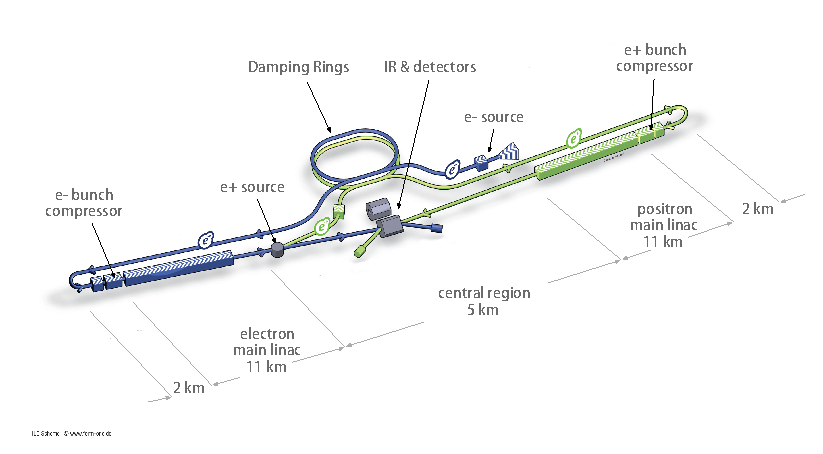
\includegraphics[width=0.85\textwidth]{ILD/ILC2}
\caption
{Schematic layout of the  International Linear Collider, indicating all the major subsystems (not to scale), taken from \cite{Behnke:2013lya}.}
\label{fig:detectorILC}
\end{figure}

\begin{figure}[tbph]
\centering
  \begin{subfigure}[t]{0.45\textwidth}
    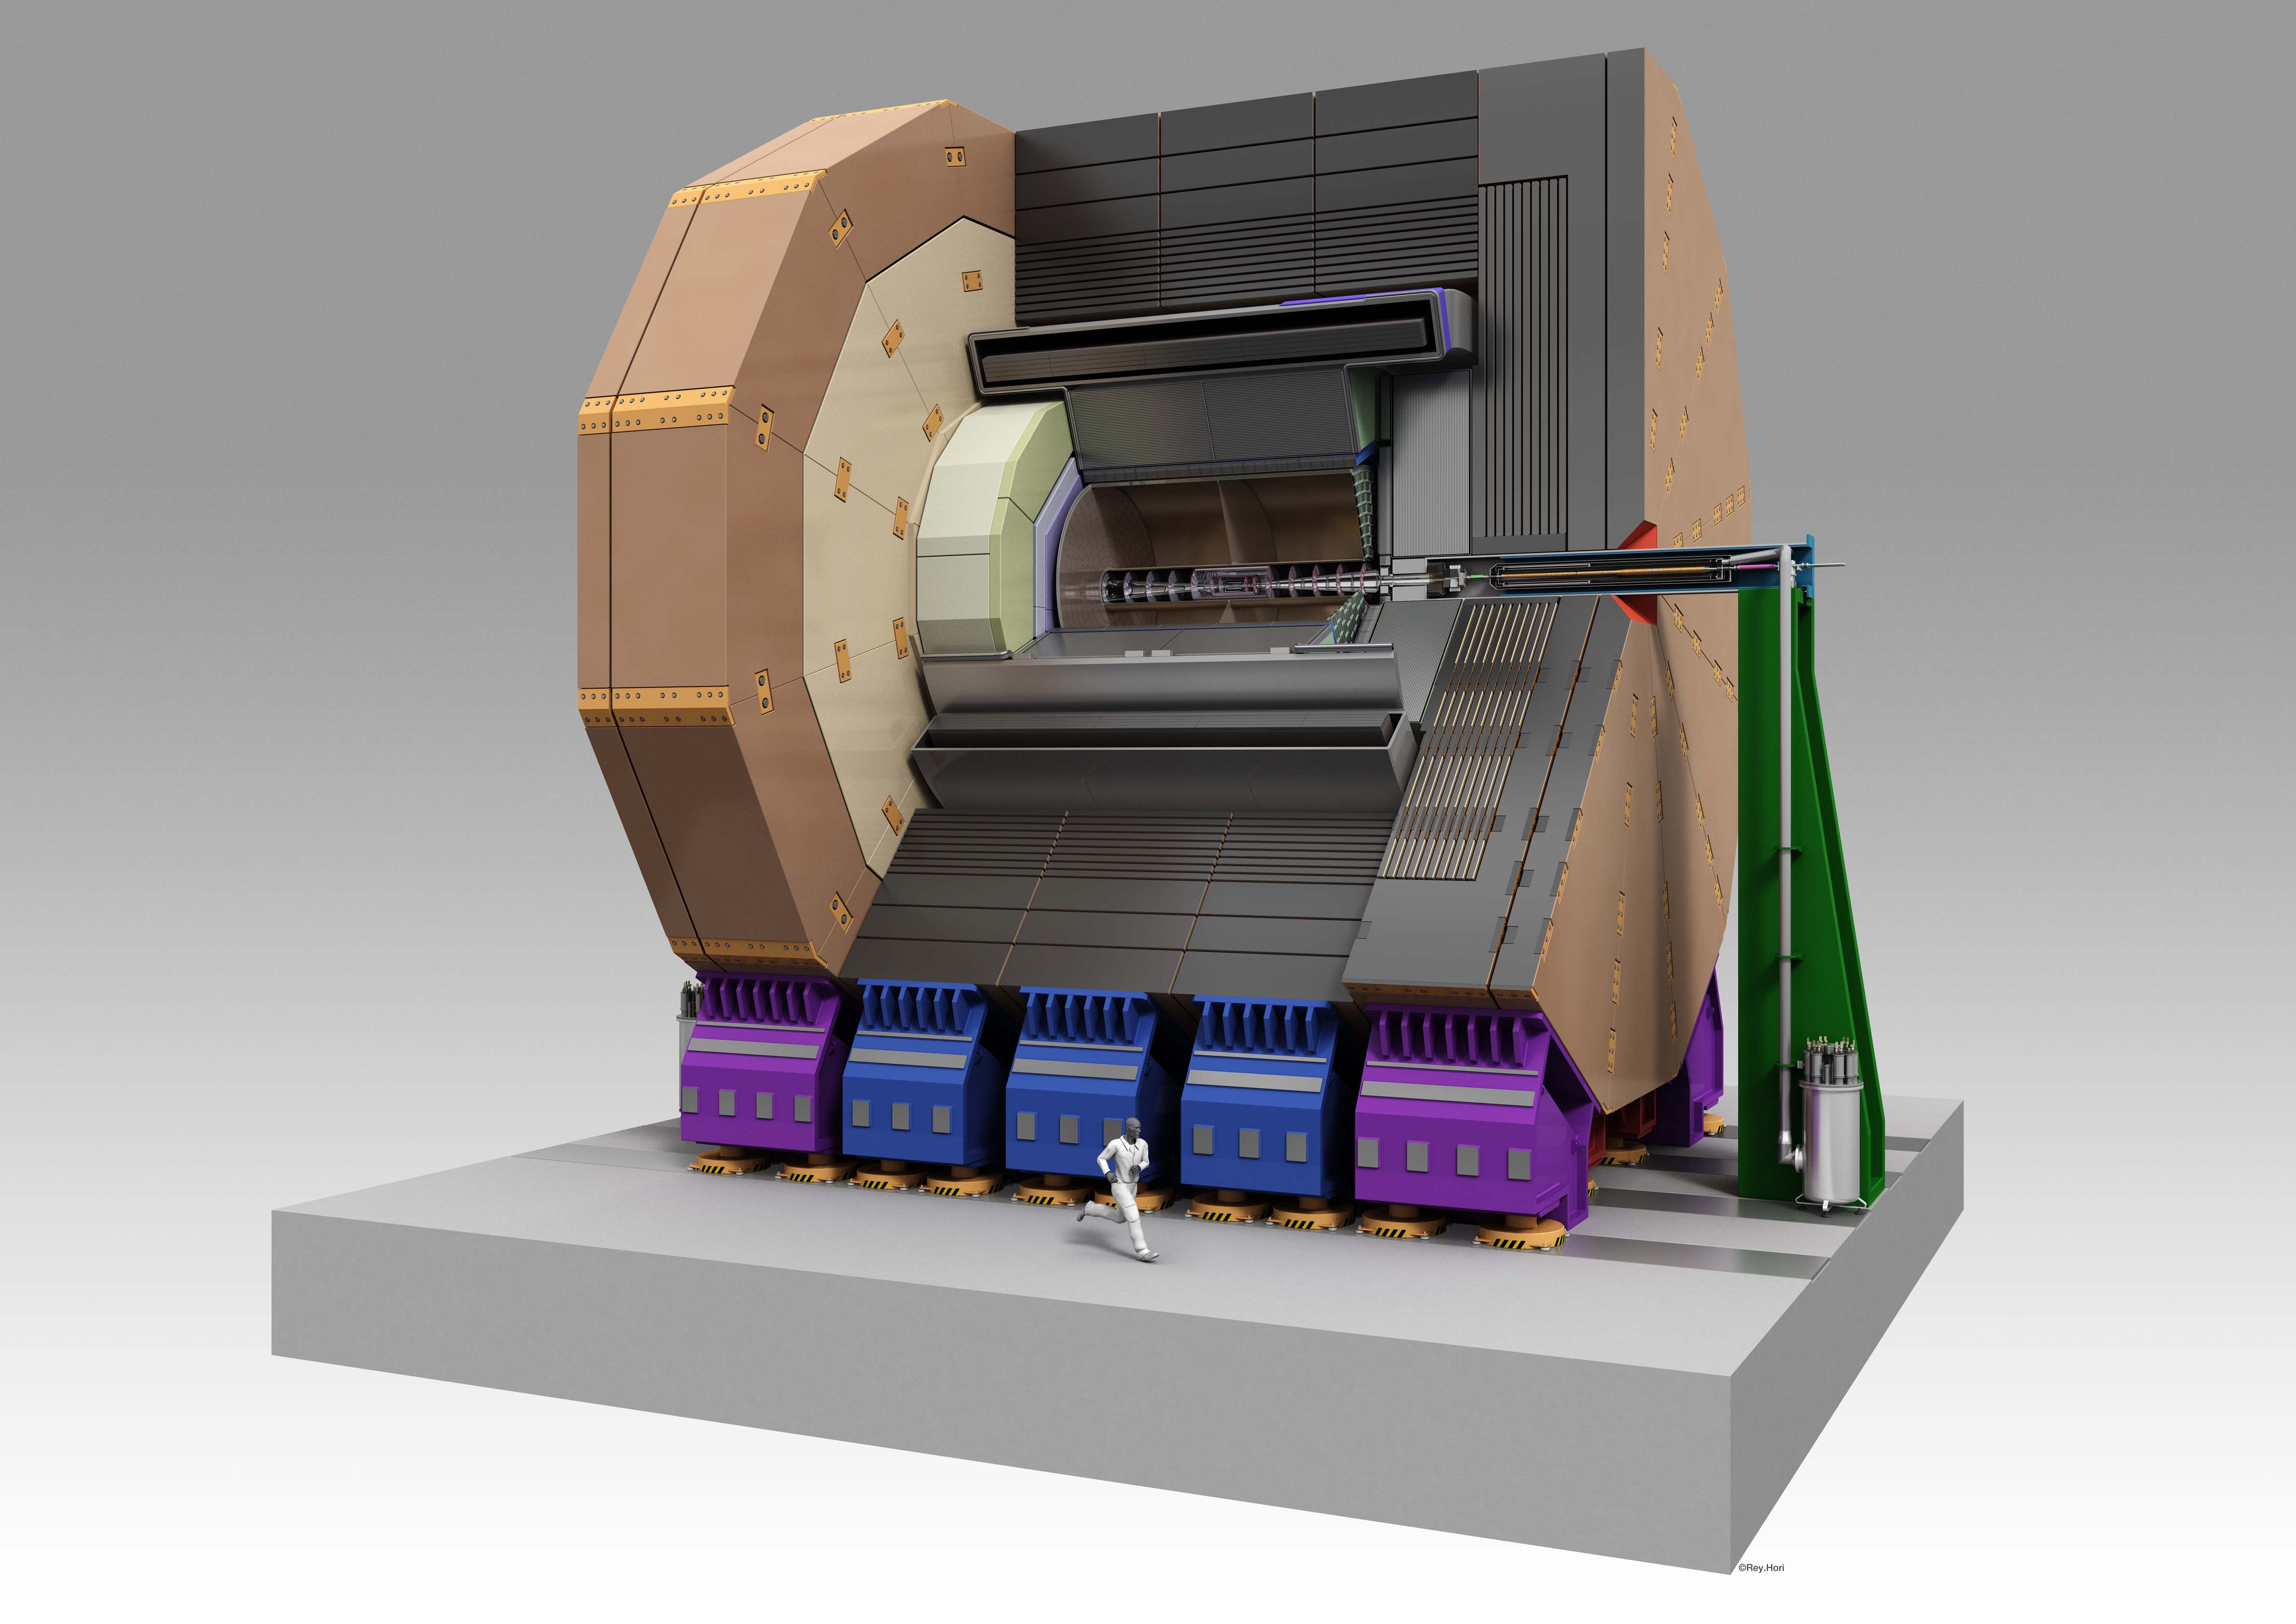
\includegraphics[width=\textwidth]{ILD/ILDview}
    \caption{}
    \label{fig:ILDview}
  \end{subfigure}
  \begin{subfigure}[t]{0.46\textwidth}
    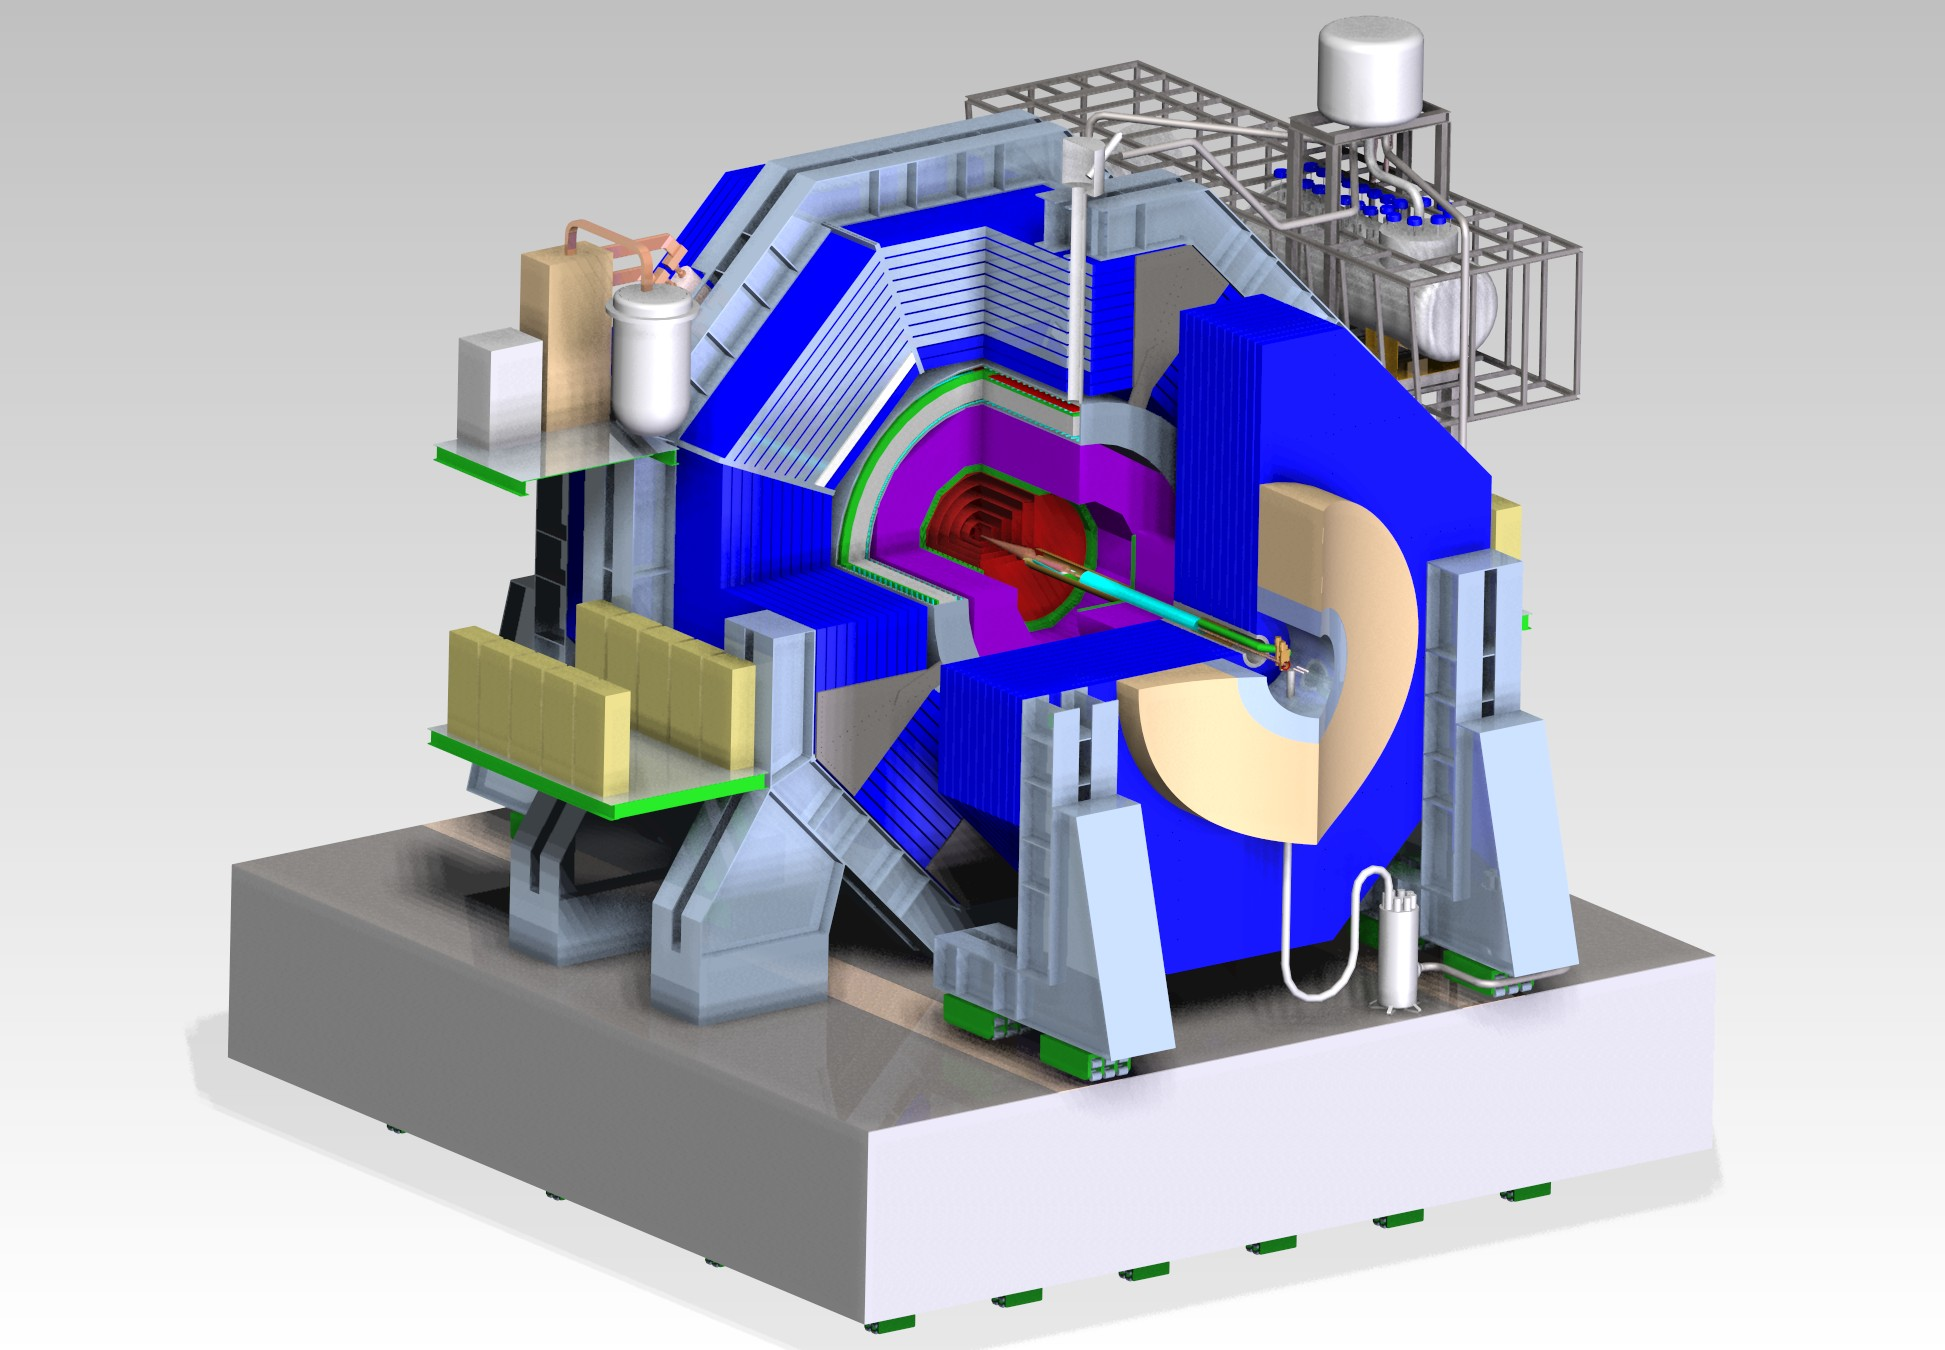
\includegraphics[width=\textwidth]{ILD/SiD}
    \caption{}
    \label{fig:SiDview}
  \end{subfigure}
\caption[International Large Detector and the Silicon Detector for the International Linear Collider.]
{a) the International Large Detector, and b) the Silicon Detector. Both detector concepts are developed for the International Linear Collider. Both figures are  taken from \cite{Behnke:2013lya}.}
\label{fig:detectorILDSiD}
\end{figure}


\begin{comment}
The International Linear Collider (ILC) is a high-luminosity linear electron-positron collider based on
1.3 GHz superconducting radio-frequency (SCRF) accelerating technology. Its centre-of-mass-energy
range is 200�C500 GeV (extendable to 1TeV). A schematic view of the accelerator complex, indicating
the location of the major sub-systems, is shown in Fig. 3.1:

The International Linear Collider (ILC) is a 200�C500 GeV (extendable to 1TeV) centre-of-mass highluminosity
linear electron-positron collider, based on 1.3 GHz superconducting radio-frequency (SCRF)
accelerating technology. Its parameters have been set by physics requirements first outlined in 2003,
updated in 2006, and thoroughly discussed over many years with the physics user community. The
physics parameters have been reviewed continuously and found to be robust to advances in the science,
including the recent discovery of a Higgs boson at the Large Hadron Collider at CERN.

The collider design is the result of nearly twenty years of R&D. The heart of the ILC, the
superconducting cavities, is based on over a decade of pioneering work by the TESLA collaboration in
the 1990s. Some other aspects were based on the R&D carried out for the JLC/GLC and NLC projects,
which were based on room-temperature accelerating structures. Since 2005, the design of the ILC
accelerator has continued as a worldwide international collaboration coordinated by the Global Design
Effort (GDE) under a mandate from the International Committee for Future Accelerators (ICFA).
Drawing on the resources of over 300 national laboratories, universities and institutes worldwide, the
GDE produced the ILC Reference Design Report (RDR) in August 2007. The work done by the GDE
during the RDR phase identified several high-risk challenges that required R&D, which have since
been the focus of the worldwide activity during the Technical Design Phase. In parallel with the
accelerator effort, detailed baseline designs of two detectors have been developed by large international
teams as a result of intense detector R&D under the coordination of the Research Directorate, also
established by a mandate of ICFA.
\end{comment}

\section{Compact Linear Collider}

\CLIC is a potential next-generation electron-positron linear particle collider at \CERN \cite{Linssen:2012hp}. \CLIC is designed to be built in three stages:  a first stage of a centre-of-mass energy of 380\,GeV; a second stage of a centre-of-mass energy of 1.4\,TeV; and the final stage of a centre-of-mass energy of 3\,TeV. The layout of the \CLIC complex at the final stage is shown in \Figure{fig:detectorCILC}.


The \ILC and  \CLIC share some common  features. Both colliders will be linear colliders as oppose to circular colliders, like the Large Hadron Collider (\LHC). Detectors for both colliders will use the high granularity particle flow calorimetry \cite{Behnke:2013lya,Linssen:2012hp}. One major difference between the two colliders is the operating energy. Due to a higher centre-of-mass energy at \CLIC, there are significant beam related backgrounds. The \ee incoherent pair background has a major influence on the design of the inner region  and the forward region of the detectors \cite{Linssen:2012hp}. The pile-up of 3.2 \ggHad background events per bunch, also integrating over 60 bunch crossings,  need to be mitigated for physics analyses  \cite{Linssen:2012hp}.  Another difference between the \ILC and  \CLIC is that the timing separation between bunches is much shorter at \CLIC. The \CLIC beam contains 312 bunch trains with a train repetition rate of 50\,Hz,  separated by 0.5\,ns between each bunch train. This short timing separation suggests that the detector will integrate over a number of bunch crossings.

%

%This, together with the significant \ggHad backgrounds, has a significant impact on the detector design.

%The beam related background needs to be suppressed in all physics analyses.


%Due to the high energy of the beam in the \CLIC, reducing the photon-photon collision background would be a major consideration for the \CLIC detector.

%Another difference is that the separation of brunch crossing in the CLIC is shorter than it is in is the ILC.


%Although the accelerating systems would be different, the calorimeter designs are similar, both highly granular for the optimal particle flow.
% is motivated by the physics reach of detecting new physics  and measuring rare decays of Higgs
% Due to the similarities of the two linear collider programmes, the development with the \CLIC detector concepts started with the \ILC detector concepts. Two  \CLIC detector concepts, the \CLICILD and the \CLICSiD, are developed based on the \ILD and the \SiD, respectively.

\begin{figure}[tbph]
\centering
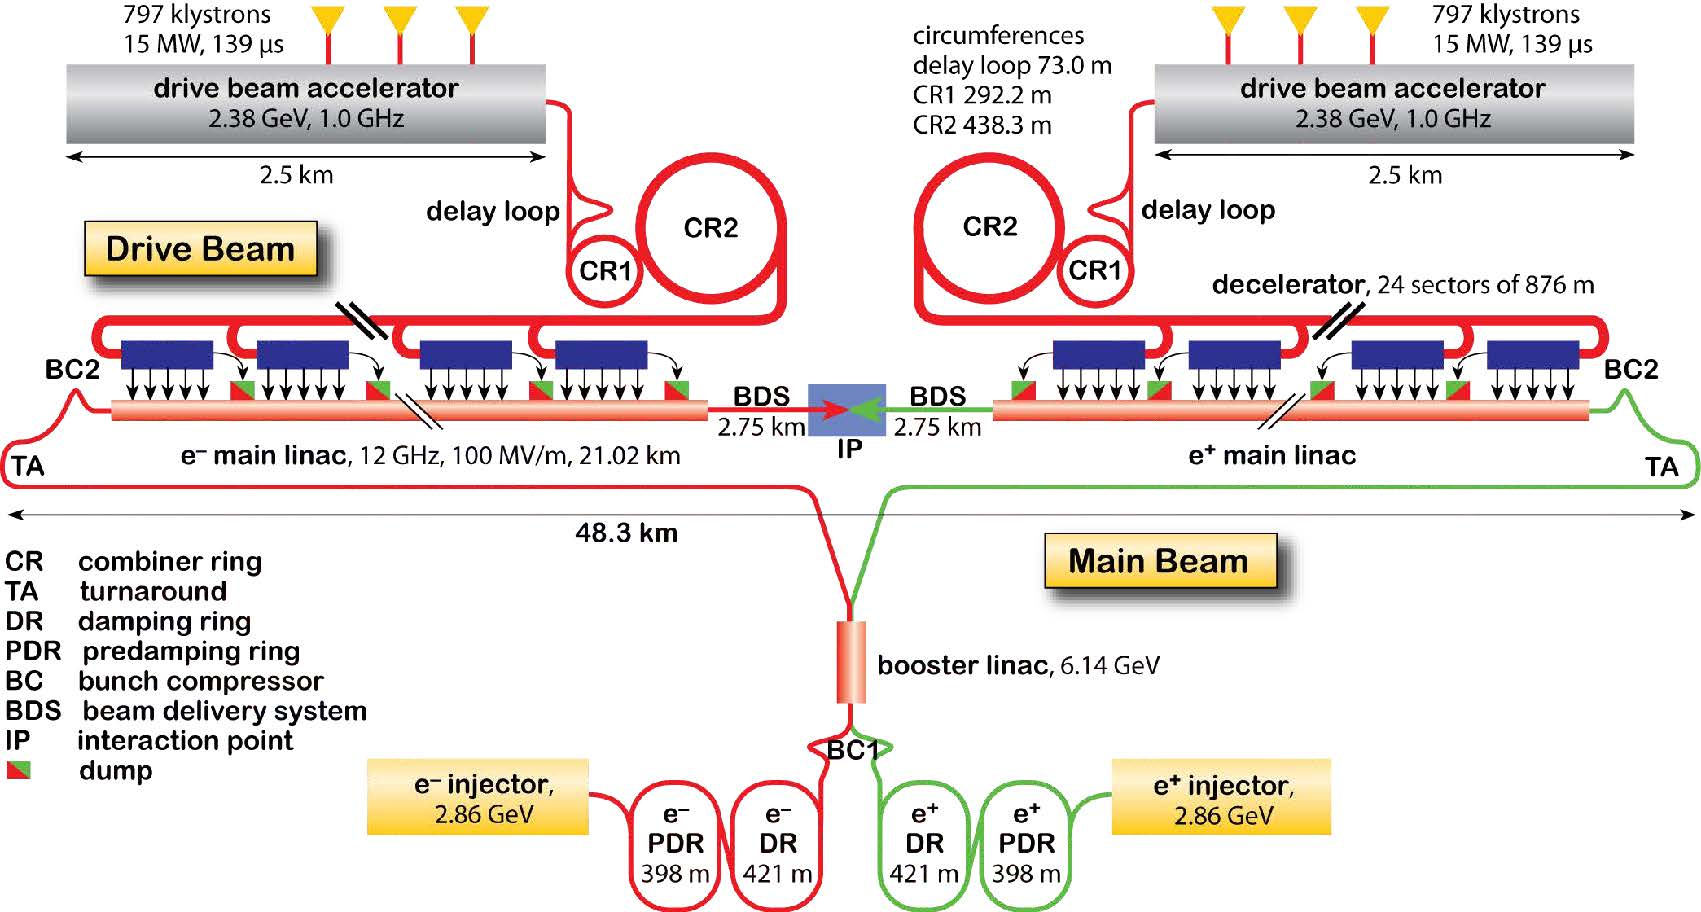
\includegraphics[width=0.85\textwidth]{ILD/CLIC}
\caption
{The layout of the Compact Linear Collider at the final stage of a centre-of-mass of energy of  3\,TeV, taken from \cite{Aicheler:2012bya}.}
\label{fig:detectorCILC}
\end{figure}

\begin{comment}
The ILC has developed two detector models, namely the International Large Detector (ILD) \cite{Abe:2010aa} and the Silicon Detector (SiD) \cite{Aihara:2010zz}. The CLIC has developed two slightly modified detector models based on ILD and SiD \cite{Linssen:2012hp}. One key common feature of these next generation electron-positron linear colliders is the high granular calorimeter, which provides a great spatial resolution at the cost of the energy resolution. Particle flow algorithms (PFA) benefit from the spatial resolution from calorimeters, together with tracking information, to provide excellent a jet energy resolution. PandoraPFA, the most complicated and the best performing one, provides a jet energy resolution of less than 3.5\%, which is required for W/Z separation \cite{Thomson:2009rp,Marshall:2013bda}.
\end{comment}





\section{Physics at future linear colliders}

An \ee linear collider has advantages over the current hadron collider, the \LHC. Those advantages include:

i) Events in the \ee collider will be cleaner than those in the hadron collider. In the \LHC, many proton$-$proton collisions per bunch crossing are expected \cite{Bruning:2004ej}, generating hundreds of particles from parton collisions. In the \ee collider, the main source of background comes from photon$-$photon collisions \cite{Brau:2007zza,Linssen:2012hp}. Depending on the operating energy and scheme, there will be only a few of these photon$-$photon collisions per bunch crossing. Particles produced from these collisions are mainly in the forward direction, which can be identified relatively easily.

ii) Electroweak interactions in the \ee collider will be democratic as the photon couples to all particles in and beyond the Standard Model equally \cite{Agashe:2014kda,Thomson:2013zua,Tong:QFT,Gripaios:GFT}. The production of pairs of all particles will be at a similar rate. In the \LHC, the non-perturbative strong interaction is the main channel for the particle production. Heavy particles has a lower production rate than light ones, as the parton distributions fall sharply for a composite object like a proton \cite{Placakyte:2011az}.

iii) In the \LHC, calculation of the cross section depends on quantum chromodynamics  and the proton structure function, which have large systematic errors. In an \ee collider, the initial particles, \Pep and \Pem, are  point-like particles, interacting through electroweak forces only. Consequently, theoretical uncertainties are smaller.

%A high theoretical precision level of the electroweak interactions could be reached.

iv) The physics at an \ee collider can be studied in detail. Without complicated underlying events, complete events can be reconstructed.  Polarised beams of electrons and positrons with known initial and final polarisation states also could be used to enhance the production of certain interactions, for example, electron$-$positron annihilation with opposite helicities.

%Reconstruction of the momenta of particle scan be calculated by kinematic fitting.

The physics programmes for the \ILC and \CLIC, which is a driving force behind the detector design, share some common features. At a centre-of-mass energy of 250\,GeV, the collider could operate as a Higgs factory, allowing measurements of precision Higgs couplings via channels like \HepProcess{\ee \to \PZ \PHiggs}. At a centre-of-mass energy of 350\,GeV, the collider can continue to measure Higgs couplings, as well as to measure top quark mass and couplings via channels such as \HepProcess{\ee \to \Ptop \APtop}.  At a centre-of-mass energy of 1\,TeV and beyond, the collider would be able to produce rare Higgs decays, allowing measurements of Higgs self-couplings and probing composite Higgs sector, and to search for supersymmetric particles.

% can continue to measure Higgs couplings, as well as to measure top quark mass and coupling with channels such as \HepProcess{\ee \to \Ptop \APtop}.

%\ILC has a reach of a centre-of-mass energy from 200\,GeV to 1\,TeV, whilst \CLIC can reach a centre-of-mass energy from 350\,GeV to 3\,TeV. Both machines are capable of precision higgs coupling measurements, top mass and coupling measurements, and search for new physics such as supersymmertry particles. The \ILC can also operate at low energy to be a \PZ and a \PHiggs factory for ultra precise \PZ mass and \PHiggs mass measurements. \CLIC, on the other hand, has the advantage of a higher energy reach, which allows measurements of rare events, such as higgs trilinear self-couplings and quartic couplings.




\section{Detector requirements}
\label{sec:detectorPhysicsRequirementPandora}


Many physics processes at a future linear collider can be characterised by multi-jet final states, often with charged leptons or missing momentum associated with neutrinos. The reconstruction of the invariant masses of two or more jets is crucial for event reconstruction and event selection. At the Large Electron$-$Positron Collider (\LEP), kinematic fitting \cite{Thomson:2004zx} allowed precise invariant mass reconstruction. At a future linear collider, reconstruction invariant mass of multiple jets for final states with missing momentum will rely heavily on the intrinsic jet energy resolution of the detector.


One goal of jet energy resolution at a future linear collider is to be able to separate  \PW and \PZ bosons, by reconstructing their invariant massese via quark-jets using the hadronic decay channel. The idealised reconstructed \PW and \PZ boson masses distributions for different jet mass resolutions are shown in \Figure{fig:detectorWZseparation}. As the invariant mass resolution is comparable to the gauge boson widths, i.e. $\sigma_m/m\approx\Gamma_{\PW}/m_{\PW}\approx\Gamma_{\PZ}/m_{\PZ}$, a separation of 2.5$\sigma$ in the masses distributions implies a jet energy resolution of 3.5\% \cite{Thomson:2009rp} for a range of jet energies from 50\,GeV to 1\,TeV.

%The physics goal of jet energy resolution at the \ILC and the \CLIC is to separate \PW and \PZ, using \Wqq and \Zqq channels, by reconstructing the invariant mass via quark-jets \cite{Baer:2013cma,Linssen:2012hp}. This translates to a requirement of 3.5-5\% of the jet energy resolution.



\begin{figure}[tbph]
\centering
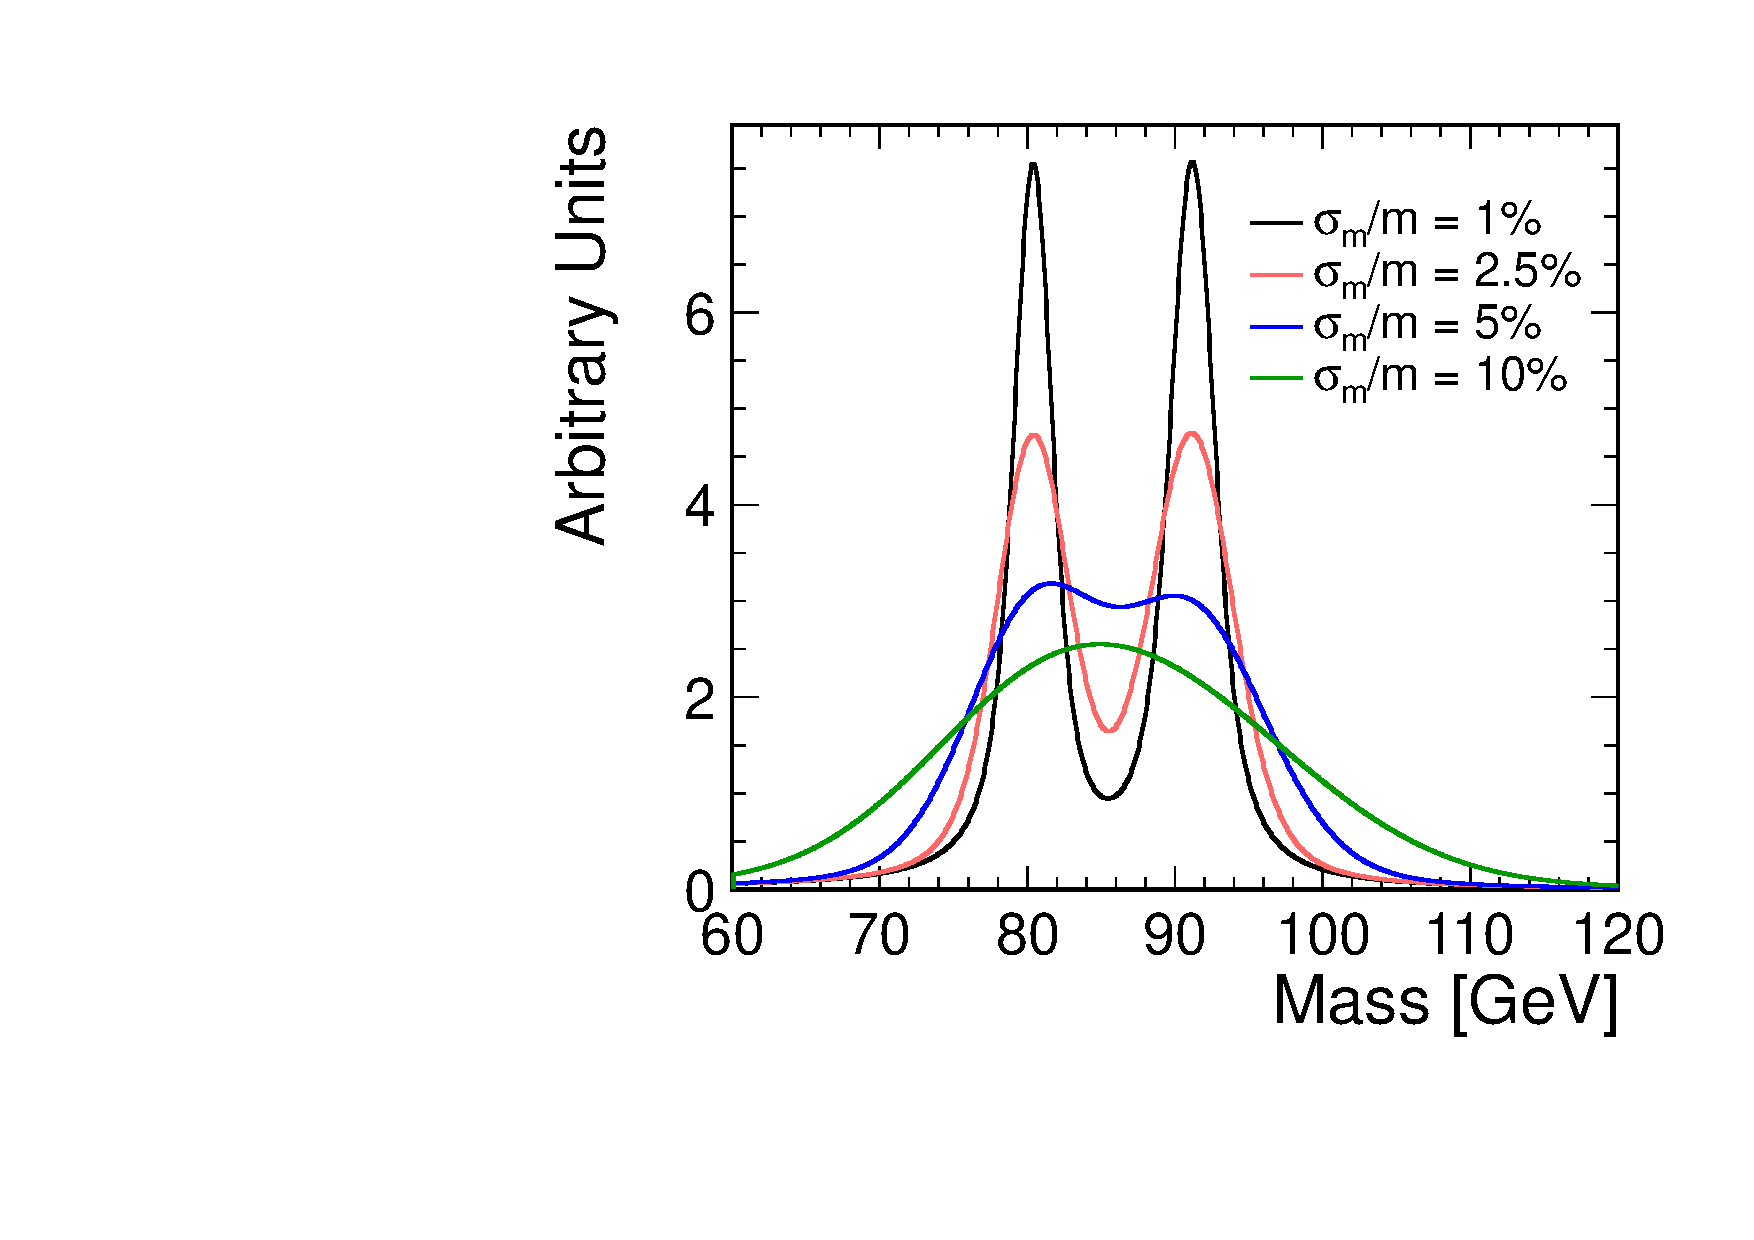
\includegraphics[width=0.45\textwidth]{{ILD/wzSeparation.pdf}}
\caption
{Ideal \PW/\PZ boson mass separation for different jet mass resolutions obtained using a Gaussian smearing of Breit$-$Wigner distribution, taken from \cite{Linssen:2012hp}.}
\label{fig:detectorWZseparation}
\end{figure}



\section{Particle Flow Calorimetry}


A jet energy resolution of 3.5\% is unlikely to be achieved with a traditional calorimeter design. Traditionally, jet energies are measured as a sum of energies deposited in the electromagnetic  (\ECAL)  and hadronic calorimeter (\HCAL), giving a jet energy resolution of the form
\begin{equation}
\frac{\sigma_{E}}{E} = \frac{\alpha}{\sqrt{E(\text{GeV})}}\oplus\beta .
\end{equation}
The stochastic term $\alpha$ is typically greater than 60\% \cite{Abe:2010aa,Behnke:2013lya}, and the constant term $\beta$ is a few percent \cite{Abe:2010aa,Behnke:2013lya}. To achieve a jet energy resolution of 3.5\% or better, the stochastic term should be less than 30\% with a small constant term, which is unlikely to be achieved by a traditional calorimeter.

%On the contrary, the particle flow approach to calorimetry  has demonstrated it ability to reach the goal \cite{Thomson:2009rp,Marshall:2012ry}.


In a typical jet, about 62\% of the jet energy is from charged particles, 27\% from photons, 10\% from long-lived neutral hadrons, and 1.5\% from neutrinos \cite{Knowles:1997dk,green1998electron}. In a traditional approach to calorimetry, the jet energy resolution is limited by the relatively poor energy resolution of the hadronic calorimeters.

The particle flow approach to calorimetry improves the jet energy resolution by fully reconstructing  all visible particles in the detector. The jet energy is the sum of energies of individual particles, where the energies of the charged particles are measured in the tracking detectors, and the energies of neutral particles are measured in calorimeters. Hence the hadronic calorimeter only measures about 10\% of the jet energy.

As shown in \Table{tab:detectorJetComponent}, assuming 30\% of the jet energy (photon energy) is measured with ${\sigma_{E}}/{E} = 15\% / \sqrt{E(\text{GeV})}$, and 10\% of the jet energy (hadron energy) is measured with ${\sigma_{E}}/{E} = 55\% / \sqrt{E(\text{GeV})}$ \cite{Behnke:2013lya}, a jet energy resolution of ${\sigma_{E}}/{E} = 19\% / \sqrt{E(\text{GeV})}$ can be obtained. This satisfies the jet energy resolution requirement for separating \PW and \PZ bosons via their hadronic decays. In reality, this level of performance is unattainable due to incorrect association of energy deposits to particles. At jet energies beyond tens of GeVs, results from imperfect reconstruction rather than the intrinsic detector performance limit the particle flow performance \cite{Thomson:2009rp}.

\begin{table}[htbp]
\small
\centering
\smallskip
\begin{tabular}{l  l r r r }
\hline
\hline
 Component &  Detector & Energy fraction & Energy resolution & Jet energy resolution \\
\hline
Charged particles (\charge) & Tracker  & $\sim0.6E_j$ & $10^{-4}E^2_{\charge}$ & < $3.6 \times 10^{-5} E^2_j$ \\
Photons (\Pphoton) & \ECAL  & $\sim0.3E_j$ & 0.15$\sqrt{E_{\Pphoton}}$ & 0.08$\sqrt{E_{j}}$ \\
Neutral hadrons(\neutral) & \HCAL  & $\sim0.1E_j$ & 0.55$\sqrt{E_{\neutral}}$ & 0.17$\sqrt{E_{j}}$ \\
\hline
\hline
\end{tabular}

\caption
{Contributions from different particle components to the jet energy resolutions (all energies in GeV). The table lists the approximate fractions of charged particles, photons, and neutral hadrons in a jet of energy $E_j$, and the assumed single particle energy resolutions. The table is adapted from \cite{Thomson:2009rp}.}
\label{tab:detectorJetComponent}
\end{table}



In the particle flow approach to calorimetry, the sum of calorimeter energies is replaced by a complex pattern-recognition problem, which is solved by the Particle Flow reconstruction Algorithm (PFA). Detailed simulations of the \ILC and the \CLIC detector concepts using the \pandora \cite{Thomson:2009rp,Marshall:2012ry} particle flow reconstruction algorithms have demonstrated that a jet energy resolution of approximately 3\% can be achieved for jet energies in the range of 100\,GeV to 1\,TeV.


%Particle flow approach to event reconstruction has shown to deliver the best possible jet reconstruction with proof-of-principle implementations such as \pandora \cite{Thomson:2009rp,Behnke:2013lya}.

Particle flow calorimetry works by fully reconstructing particles and associating calorimeter hits to tracks in tracking detectors. This places stringent requirements on the calorimeter designs.  The \ECAL and the \HCAL need to be highly granular for an excellent spatial resolution to correctly associate calorimeter hits to the inner detector tracks. The tracking system needs to have an excellent momentum resolution for the momentum measurements of the charged particles.

\begin{comment}

The particle flow calorimetry requires to fully reconstruct particles and to associate calorimeter hits to tracks in tracking detectors. This is a demanding task for the software design and the detector design. The software details of the \pandora, which is a successful particle flow implementation, are described in \Section{sec:pandoraPandoraPFA}. For the detector design, the detector needs to be highly granular for an excellent spatial resolution, which is needed to correctly associate calorimeter hits to the inner detector tracks. This imposes stringent requirements in the \ECAL and the \HCAL designs.


 %and it is illustrated with a brief description of the particle flow principle.

\begin{figure}[tbph]
\centering
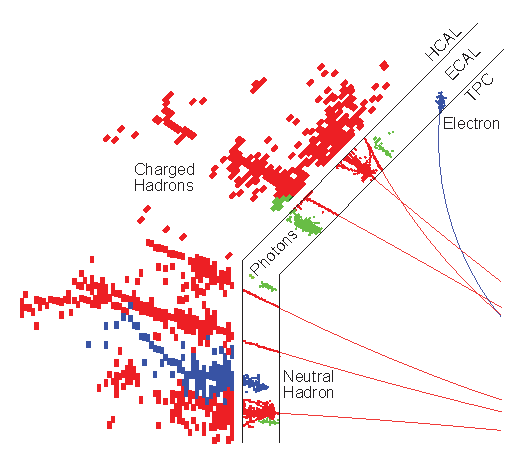
\includegraphics[width=0.45\textwidth]{{ILD/jetCLIC_ILD}}
\caption[A typical topology of a 250\,GeV jet.]
{A typical topology of a 250\,GeV jet, simulated with thr \CLICILD detector concept, taken from \cite{Marshall:2012ry}.}
\label{fig:detectorJetCLICILD}
\end{figure}


\FIGURE{fig:detectorJetCLICILD} shows a typical topology of a 250\,GeV jet, simulated with the \CLICILD detector concept. Particles consisting of the calorimeter hits and tracks are labelled with different colours. Clusters of calorimeter hits in the highly granular \ECAL and \HCAL are associated with tracks from the inner tracking detector, time projection chamber (\TPC). Photons are identified using the characteristics longitudinal and transverse electromagnetic shower profiles. Hadronic showers are separated from electromagnetic showers due to the small transverse spread of the electromagnetic shower.  The inner tracking detector should be highly efficient and have very little material. For the calorimeter, the \ECAL and \HCAL, both should be highly granular. The material of the calorimeter should be dense and has a large ratio of interaction length to radiation length.
\begin{comment}
\subsection{Other requirements on the detector design}

Other physics requirements for the detectors for the \ILC and the \CLIC are summarised in \cite{Baer:2013cma,Linssen:2012hp}. Here important requirements are presented as motivations for detector designs.


The performance requirement of the vertex detector is determined by the required performance of b-quark and c-quark tagging. The ability to identify secondary vertices and tracks, which are not originated from the interaction point, is the prerequisite for the flavour tagging. The impact parameter resolution can be written in the form of:
\begin{equation}
\sigma_{d_0}^2 = a^2 + \frac{b^2}{p^2\sin^2\left(\theta\right)},
\end{equation}
where $a$ is related to the point resolution and $b$ is related to multiple scattering. The requirements for both the \ILC and the \CLIC detectors are $a \lesssim 5 \mu{m}$ and $b \lesssim 15 \mu{m}\,GeV$ \cite{Behnke:2013lya,Linssen:2012hp}.


The requirement of tracking momentum resolution is driven by the Higgs boson mass resolution via the Higgsstrahlung process, \eeTo{\PZ \PHiggs}. The Higgs mass can be reconstructed precisely as the recoil mass against the \PZ momenta, which is obtained via \HepProcess{\PZ \to \APmuon \Pmuon}. For the \ILC operating at \rootSGeV{250}, the momentum resolution needs to be  $\sigma_{\pT} / \pT^2 \lesssim 5 \cdot 10^{-5}$\,\uprightMath{GeV^{-1}} \cite{Behnke:2013lya}. For the \CLIC at a higher  centre-of-mass energy, the momentum resolution needs to be  $\sigma_{\pT} / \pT^2 \lesssim 2 \cdot 10^{-5}$\,\uprightMath{GeV^{-1}} \cite{Linssen:2012hp}.

The lepton identification should be over 95\% for effective lepton tagging. The forward converge of the detector should be down to a very low angle, i.e. a few mrad, with respect to the beam axis. This is more critical for the \CLIC as particles are boosted at a high centre-of-mass energy.
\end{comment}

\section{International Large Detector}

Two detector concepts have been developed for the \ILC. The motivation for having two detectors is to have multiple independent measurements within one collider for cross-checking, complementarity, and competition between collaborations. The two detectors are both designed to be general purpose detectors. The Silicon Detector, \SiD \cite{Aihara:2010zz}, is a compact detector with silicon tracking modules and a magnetic field of 5\,T. The other detector, the International Large Detector, \ILD \cite{Abe:2010aa}, is a larger detector with a time projection chamber as the main tracking detector.

%A view of the \ILD and the \SiD detector concepts can be seen in \Figure{fig:detectorILDSiD}
% Both detectors have highly granular calorimeters optimised for the particle flow.

%Precision tests for the Standard Model requires an excellent jet energy resolution and mass reconstruction. Particle low algorithms (PFA), based event reconstruction, meet the requirements. For the best performance of the PFA, high granular calorimeter systems and highly efficient tracking systems are needed. The requirement to separate \PW and \PZ bosons in hadronic decay final states requires a jet energy resolution below 3.5\%. The momentum resolution of $5\times10^{-5}$\,GeV is motivated by the Higgs boson recoil reconstruction in the Higgsstrahlung.




The \ILD detector concept has been optimised for particle flow techniques. \FIGURE{fig:ILD} shows the longitudinal cross section of top quadrant of the \ILD detector concept. From the interaction point (\IP) outwards, there is: a tracking system comprising a large time projection chamber (\TPC) augmented with silicon tungsten layers; highly granular electromagnetic calorimeters (\ECAL) and hadronic calorimeters (\HCAL);  forward calorimeters (\FCAL); a superconducting solenoid; and muon chambers embedded within the iron return yokes. The key parameters of the \ILD are listed in \Table{tab:ILDvsCLICILD}. The section below describes the sub-detectors of the \ILD detector concept referred to as the ILD\_o1\_v05 option in the \Mokka detector simulation \cite{MoradeFreitas:2002kj}, used for the \ILD technical design report\cite{Behnke:2013lya}.



%This is a demanding task for the software design and the detector design. The software details of the \pandora, which is a successful particle flow implementation, are described in \Section{sec:pandoraPandoraPFA}. For the detector design, the detector needs to be highly granular for an excellent spatial resolution, which is needed to correctly associate calorimeter hits to the inner detector tracks. This imposes stringent requirements in the \ECAL and the \HCAL designs.


%This detector concept has been optimised \cite{Abe:2010aa} and used in studies described in subsequent chapters.




%The particle flow paradigm requires topological information of individual particle reconstructions. The sub-detector systems need to have the spatial resolution to separate charged particles from neutral particles. The result is a highly granular calorimeter and a central tracking system with excellent momentum resolution.



%The \CLICILD detector concept for the \CLIC in the conceptual design report\cite{Linssen:2012hp} is a modified version of the \ILD, adapted to the \CLIC colliding environment. As they share similarities, an overview of the \ILD sub-detectors is provided, followed by a discussion on the difference between the \ILD and the \CLICILD detector concepts.  A comparison of the longitudinal cross section of the top quadrants of between \ILD and \CLICILD can be seen in \Figure{fig:detectorILD}.


\begin{figure}[tbph]
\centering
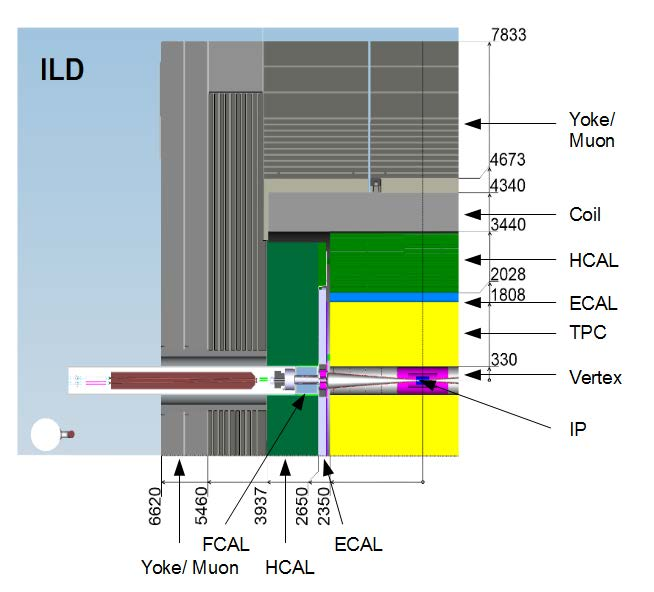
\includegraphics[width=0.85\textwidth]{ILD/ILD}
\caption
{The longitudinal cross section of top quadrant of the \ILD, taken from  \cite{Behnke:2013lya}. From interaction point (\IP) outwards, there is: a tracking system comprising a large time projection chamber (\TPC) augmented with silicon tungsten layers; highly granular electromagnetic calorimeters (\ECAL) and hadronic calorimeters (\HCAL);  forward calorimeters (\FCAL); a superconducting solenoid; and muon chambers embedded within the iron return yokes. The dimensions are in units of mm.}
\label{fig:ILD}
\end{figure}


\begin{table}[htbp]
\centering
\smallskip
\begin{tabular}{l  r  r }
\hline
\hline
Component &  \ILD & \CLICILD \\
\hline
Tracker & TPC; Silicon & TPC; Silicon \\
Solenoid Field & 3.5\,T & 4\,T \\
Solenoid Field Bore & 3.3\,m & 3.4\,m \\
Solenoid Length & 8.0\,m & 8.3\,m \\
\VTX Inner Radius  & 16\,mm & 31\,mm \\
\ECAL $r_{min}$ & 1.8\,m & 1.8\,m \\
\ECAL $\Delta{r}$  & 172\,mm & 172\,mm \\
\HCAL Absorber Barrel / Endcap & Fe / Fe & Fe / W \\
\HCAL Interaction Length & 5.5\,\uprightMath{\lambda_I} & 7.5\,\uprightMath{\lambda_I} \\
Overall Height  & 14.0\,m & 14.0\,m \\
Overall Length  & 13.2\,m & 12.8\,m \\
\hline
\hline
\end{tabular}

\caption[A comparison of key parameters of the \ILD and \CLICILD detector concepts.]
{A comparison of key parameters of the \ILD and \CLICILD detector concepts. \ECAL $r_{min}$ is the smallest distance from the calorimeter to the main detector axis. The table is adapted from \cite{Linssen:2012hp}.}
\label{tab:ILDvsCLICILD}
\end{table}



\begin{comment}
The ILC has been designed to enable two experiments (SiD and ILD) sharing one interaction region using
a push-pull approach. This two-detector design is motivated by the enhanced scientific productivity of
past collider facilities which benefited from independent operation of multiple experiments, providing
complementary strengths, cross-checking and confirmation of results, reliability, insurance against
mishaps, competition between collaborations, as well as increased number of involved scientific
personnel. Figure 4.1 shows the arrangement of the two detectors in the detector hall.
Both detector designs are conceived as multi-purpose detectors, optimised for the broad range
of physics opportunities at the ILC. SiD is a compact, cost-constrained detector made possible
with a 5 Tesla magnetic field and silicon tracking. Silicon enables time-stamping on single bunch
crossings to provide robust performance, derived from immunity to spurious background bursts. The
highly granular calorimeter is optimised for particle-flow analysis. The ILD group has designed a
large detector with robust and stable performance over a wide range of energies. The concept uses
a tracking system based on a continuous-readout time-projection chamber combined with silicon

In order to realise the physics programme, the ILC detectors face challenges requiring significant advances
in collider detector performance. The machine environment is benign by LHC standards, enabling
designs and technologies that are unthinkable at the LHC. However, the ILC environment poses its
own set of background issues that must be overcome. The ��Detailed Baseline Design�� of the SiD and
ILD detectors have been developed to achieve the requirements for all considered physics programmes,
over the full range of centre-of-mass energies from 200 GeV up to 1TeV, as well as the possibility of
special running at the Z-pole.
The ILC physics opportunities place a premium on high-resolution jet energy reconstruction and
di-jet mass performance. Event reconstruction techniques based on the Particle Flow Algorithm (PFA)
have been developed to meet this challenge. This motivates highly granular electromagnetic and hadron
calorimeters and highly efficient tracking systems. New detector technologies and new reconstruction
algorithms based on the PFA approach achieve the needed precision in the reconstruction of jets of 3
to 4 percent for 100 GeV jets, set by the requirement to separate W and Z di-jet final states. The
requirements on momentum resolution for charged tracks (p/p2 of 5 �� 10.5 (GeV/c).1) are driven
by reconstruction of a Higgs boson recoiling from the associated Z boson decaying to a lepton pair in
the Higgs-strahlung process. Flavour and quark-charge tagging will be available at an unprecedented
level of performance as a result of the development of a new generation of vertex detectors. Particle
identification is achieved by the highly granular calorimeters and muon identification is aided by the
instrumented iron return yoke.
A very important element of the detector design work has been the common effort to develop and
apply simulation tools to realise realistic detector-performance estimates. A small group of experts
from both SiD and ILD have cooperated closely on this critical work.
To preserve this unprecedented performance, the inner detectors must accommodate very lowmass
detectors and supports. This is a significant challenge. The detector designs have achieved the
required light-weight support structures with minimal dead spaces. This was greatly simplified by the
ILC time structure of 1 millisecond bunch trains at 5 Hertz. This very sparse filling allows power for
many of the detector subsystems to be switched off between bunch trains (so-called power pulsing),
reducing the heat load and the need for cooling. The design of these power-pulsed systems presents a
significant challenge, including the need for quiescent currents.
27
\end{comment}


%\section{\ILD sub-detectors}

%This section discusses the \ILD sub-detectors. Starting with a discussion of the precision vertex detector and the tracking system, which are closest to the interaction point, the discussion moves onto the highly granular calorimeter system of the electromagnetic and hadronic calorimeters. A discussion on solenoid, iron yoke and the muon system will be presented, followed by a discussion on the very forward calorimeters.

%The \ILD detector concept is designed as a general purpose detector. Closest to the interaction points are a precision vertex detector and a tracking system. The tracking system consists of silicon tracking components and a time projection chamber. Surrounding the tracking system is a highly granular calorimeter system. The outer solenoid provides a magnetic field of 3.5\,T. The most outer iron return yoke also acts as a muon calorimeter.


\subsection{Vertex Detector}

The pixel-vertex detector (\VTX) needs to be close to the interaction point to reconstruct secondary vertices. As the \TPC is the main tracking  detector, the \VTX mainly measures the impact parameter of tracks. \FIGURE{fig:detectorILDVXT} shows the structure of the vertex detector.  The structure is of three, nearly cylindrical, concentric layers of double-sided ladders. Each ladder contains pixel sensors on both sides at 2\,mm separation between two layers. This results in six measured  positions for each charged particle traversing the detector. The first double layer is half the length of the other two, to avoid the high occupancy region of direct low momentum hits from the incoherent pair background. The baseline geometry of the vertex detector can be found in \Table{tab:detectorVertex}.  The radii covered by the detector range from 16 mm to 60 mm.


\begin{figure}[tbph]
\centering
    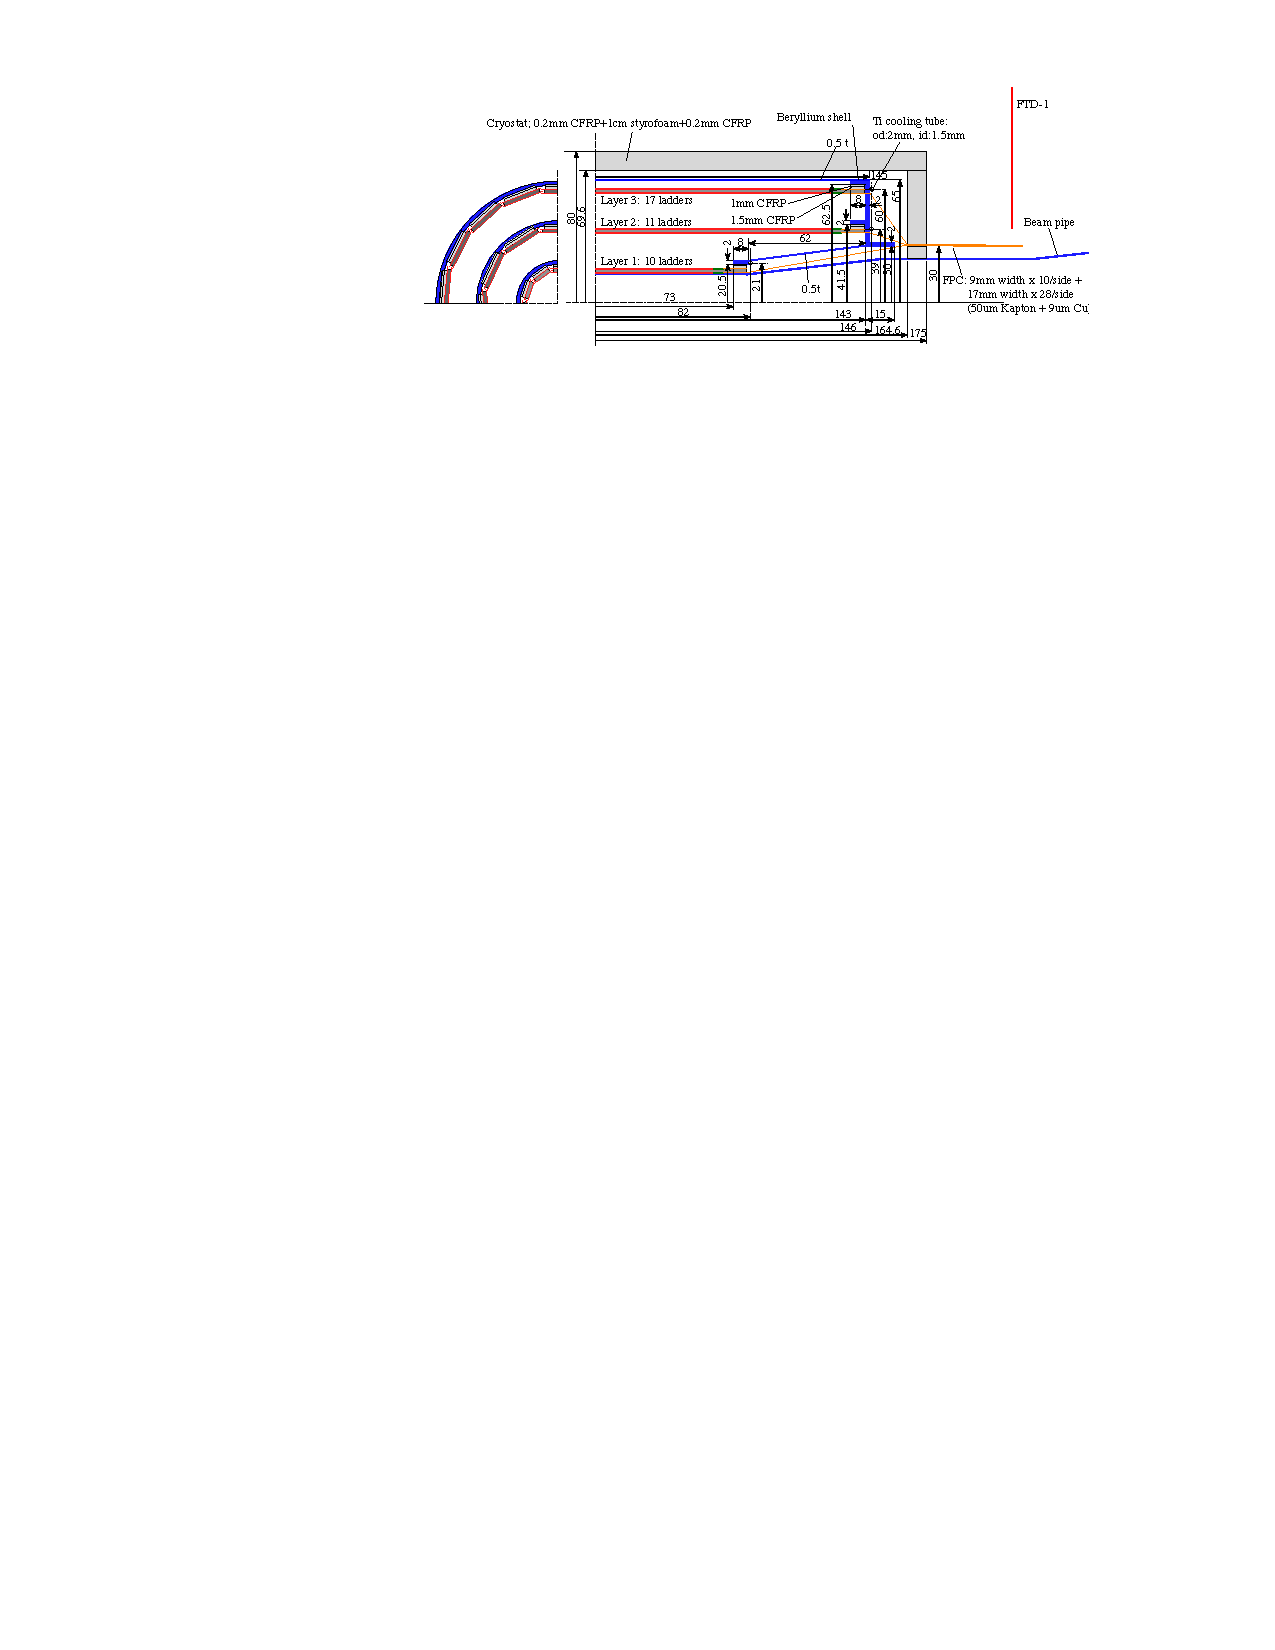
\includegraphics[width=0.85\textwidth]{{{ILD/ILD_VTX}}}
\caption
{
Structure of \ILD vertex detector, taken from \cite{Behnke:2013lya}.}
\label{fig:detectorILDVXT}
\end{figure}


\begin{table}[htbp]
\centering
\smallskip
\begin{tabular}{l  r r r r r }
\hline
\hline
 &  R & \absOf{z} & $\absOf{\cos\parenths{\theta}}$ & $\sigma$ & Readout time \\
\hline
Layer 1 & 16\,mm & 62.5\,mm & 0.97 & 2.8\,$\mu$m & 50 \,$\mu$s \\
Layer 2 & 18\,mm & 62.5\,mm & 0.96 & 6\,$\mu$m & 10 \,$\mu$s \\
\hline
Layer 3 & 37\,mm & 125\,mm & 0.96 & 4\,$\mu$m & 100 \,$\mu$s \\
Layer 4 & 39\,mm & 125\,mm & 0.95 & 4\,$\mu$m & 100 \,$\mu$s \\
\hline
Layer 5 & 58\,mm & 125\,mm & 0.91 & 4\,$\mu$m & 100 \,$\mu$s \\
Layer 6 & 60\,mm & 125\,mm & 0.90 & 4\,$\mu$m & 100 \,$\mu$s \\
\hline
\hline
\end{tabular}

\caption
{Key parameters for vertex detector in the \ILC. The spatial resolution ($\sigma$) and readout times are for the CMOS option. The table is adapted from \cite{Behnke:2013lya}.}
\label{tab:detectorVertex}
\end{table}



\subsection{Tracking Detectors}

The hybrid  tracking system consists of a large time projection chamber (\TPC), a Silicon Inner Tracker (\SIT), a Silicon External Tracker (\SET) in the barrel region, a silicon end cap tracking component (\ETD) behind the endplate of the \TPC, and a silicon forward tracker (\FTD) in the forward region.  A top quadrant view of the \ILD silicon envelope system with the \TPC is shown in  \Figure{fig:detectorTrackingFull}. The \SIT, \SET, and \ETD are made up of two single-sided strip layers tilted by a small angle. The \FTD is a system of two silicon-pixel disks and five silicon-strip disks.   The main parameters of the silicon system and the \TPC can be found in \Table{tab:detectorTracking}.

A \TPC tracking detector has several advantages: a) tracks can be measured with a large number of three-dimensional ($r,\phi,z$) spatial points; b) the continuous tracking allows precise reconstruction of tracks; and c) the \TPC uses a minimum amount of material, which minimises the photon to electron pair conversion.


%due to the $10^3$ beamstrahlung photons per bunch-crossing in the barrel region \cite{Vogel:2008zza}.

%The \TPC is optimised for point resolution and minimum material, as required for the best calorimeter performance and the best particle flow performance.

The silicon intermediate tracker (\SIT) and the silicon envelope tracker (\SET)  provide spatial point measurements before and after the \TPC in the barrel region. This helps to  improve the overall momentum resolution by providing points to link the vertex detector with the \TPC, and to extrapolate tracks from the \TPC to the calorimeters.  The \FTD improves the low angle coverage of the tracking system, where the low angle is not covered by the \TPC.


\begin{comment}
The central tracker of ILD is a Time Projection Chamber (TPC). A TPC tracker in a linear collider
experiment offers several advantages. Tracks can be measured with a large number of three-dimensional
 space points. The point resolution, point, and double-hit resolution, which are moderate when
compared to silicon detectors, are compensated by continuous tracking. The TPC presents a minimum
amount of material as required for the best calorimeter and PFA performance. A low material budget
also minimises the effects due to the  103 beamstrahlung photons per bunch-crossing which traverse
the barrel region [255]. Topological time-stamping in conjunction with inner silicon detectors is an
important tool that is explained in section 6.1.2.5. To obtain good momentum resolution and to
suppress backgrounds, the detector will be situated in a strong magnetic field of 3.5 T. Under this
condition a point resolution of better than 100 \mu m for the complete drift and a double hit resolution
of < 2 mm are possible.
Continuous tracking facilitates the reconstruction of non-pointing tracks which are significant for
the particle-flow measurement and for the reconstruction of physics signatures in many scenarios.
The TPC yields particle identification via the specific energy loss dE/dx which is valuable for many
physics analyses.



A system of silicon strip and pixel detectors surrounds the VTX detector. In the barrel, two
layers of silicon strip detectors (SIT) are arranged to bridge the gap between the VTX and the TPC.
In the forward region, a system of two silicon-pixel disks and five silicon-strip disks (FTD) provides
low angle tracking coverage.

The barrel silicon parts SIT and SET provide precise space points before and after the TPC; this
improves the overall momentum resolution, helps in linking the VTX detector with the TPC, and
in extrapolating from the TPC to the calorimeter. The coverage of the TPC with silicon tracking
is completed by the ETD, located within the gap separating the TPC and the end-cap calorimeter.
Together these systems help in calibrating the overall tracking system, in particular the TPC. The
good timing resolution of the silicon detectors relative to the time between bunches in the ILC together
with the high spatial precision helps in time-stamping tracks and assigning them to a given bunch
within an ILC bunch train.
\end{comment}





\begin{figure}[tbph]
\centering
  \begin{subfigure}[b]{0.45\textwidth}
    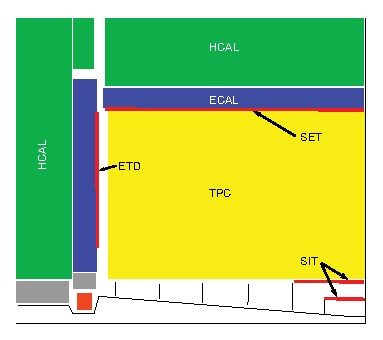
\includegraphics[width=\textwidth]{ILD/Tracking}
    \caption{}
    \label{fig:detectorTracking}
  \end{subfigure}
    \begin{subfigure}[b]{0.45\textwidth}
    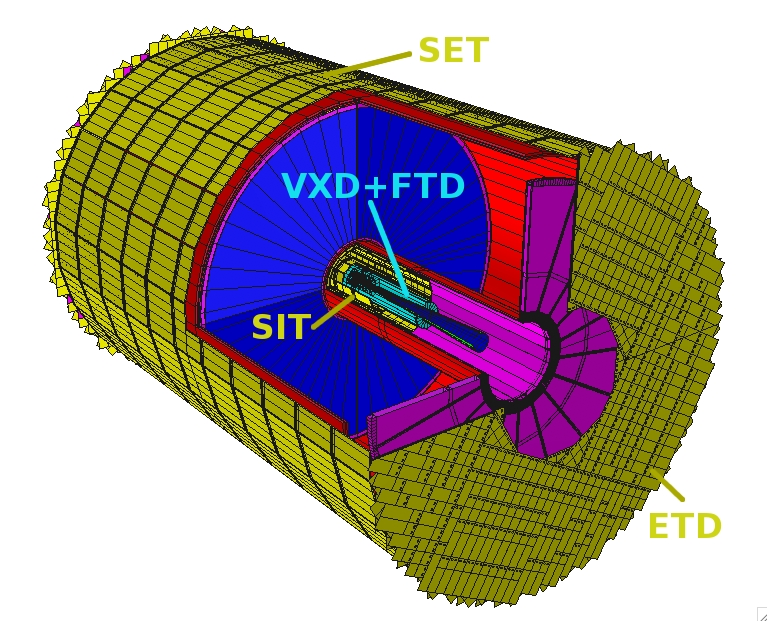
\includegraphics[width=\textwidth]{ILD/ILDtracking}
    \caption{}
    \label{fig:detectorTracking3D}
  \end{subfigure}
\caption
{a) A top quadrant view of the \ILD silicon envelope system, \SIT, \SET, \FTD, and \ETD, with \TPC, \ECAL, and \HCAL, and b)  a 3D detailed GEANT 4 simulation description of the
silicon system as sketched in the quadrant view in a). Both plots are adapted from figures in \cite{Behnke:2013lya}.}
\label{fig:detectorTrackingFull}
\end{figure}


\begin{table}[htbp]
\centering
\smallskip
\begin{tabular}{l  r r r }
\hline
\hline
 &  R & z & ${\cos\parenths{\theta}}$ \\
\hline
SIT & 153\,mm & 368\,mm & 0.910 \\
SIT & 300\,mm & 644\,mm & 0.902 \\
SET & 1811\,mm & 2350\,mm & 0.789 \\
ETD & 419 - 1822.7\,mm & 2420\,mm & 0.985 - 0.799 \\
\hline
TPC  & 329 - 1808\,mm & $\pm$2350\,mm & up to 0.98 \\
\hline
\hline
\end{tabular}

\caption
{Main parameters of the central silicon tracking systems (SIT, SET, and ETD) and the TPC. The table is adapted from \cite{Behnke:2013lya}.}
\label{tab:detectorTracking}
\end{table}



\subsection{Electromagnetic Calorimeter}

The silicon$-$tungsten sampling electromagnetic calorimeters in  the \ILD consist of an octagonal barrel and two end cap systems. The fine granularly \ECAL is located inside the \HCAL. Both \ECAL and \HCAL are inside the superconducting solenoid. \FIGURE{fig:detectorILDECAL2} shows the position of the electromagnetic calorimeter in the \ILD detector and the trapezoidal form of the modules.

% The \ECAL measures photon energies and separates photons from other particles. The \ECAL also hosts the first part of the hadronic showers and greatly assists the separation of hadronic showers.

The particle flow paradigm has a large impact on the \ECAL design. In addition to measuring and separating photons, the \ECAL needs to allow the  reconstruction of  detailed shower profiles to separate electromagnetic showers from hadronic showers, as approximately 50\% of hadronic showers start in the \ECAL.

%These requirements can be fulfilled with an excellent three-dimensional granular \ECAL.

From test beam data and simulation studies \cite{Ramilli:2012dva,Adloff:2009zz,Adloff:2013jqa}, a sampling calorimeter with a longitudinal segmentation below one radiation length and the transverse segmentation respectively below one Moli\`{e}re radius  is required. A compact design is realised with tungsten as the absorber material and silicon pad diodes as the active material. A cross section of an \ECAL layer is shown in \Figure{fig:detectorILDECAL}. Tungsten is a dense material with a large ratio of interaction length to radiation length. A small radiation length will promote the start of the electromagnetic shower earlier in the calorimeter, whilst a large interaction length will reduce the fraction of hadronic showers starting in the \ECAL.

The \ECAL, which is about 20\,cm thick, has  30 longitudinal layers providing about 24 radiation lengths. The first 20 layers use 2.1\,mm thick absorber plates and the last 10 layers have 4.2\,mm   thick absorber plates.

%The test beam data with electrons shows the energy resolution of the \ECAL concept to be $16.6/\sqrt{E(\ GeV)}\oplus1.1\%$ \cite{Behnke:2013lya}, which is compatible with the values assumed for the full \ILD detector simulation.

The choice of thin silicon layers offers a great spatial resolution. The chosen size of 5.1$\times$5.1\,\uprightMath{{mm}^2} silicon pads provides enough segmentation to meet the requirements of the particle flow paradigm.



 %at a cost of the energy resolution in favour of the particle flow.








%The longitudinal segregation is a compromise between the cost and the performance. The total of 30 layers, which is about 20\,cm, provides about 24 radiation lengths. The first 20 layers use 2.1\,mm thick absorber plates, which is twice finer sampling than the last 10 layers with 4.2\,mm   thick absorber plates. The test beam data with electrons shows the energy resolution of the \ECAL concept to be $16.6/\sqrt{E(\ GeV)}\oplus1.1\%$ \cite{Behnke:2013lya}, which is compatible with the values assumed for the full \ILD detector simulation.




\begin{figure}[tbph]
\centering
    \begin{subfigure}[b]{0.48\textwidth}
        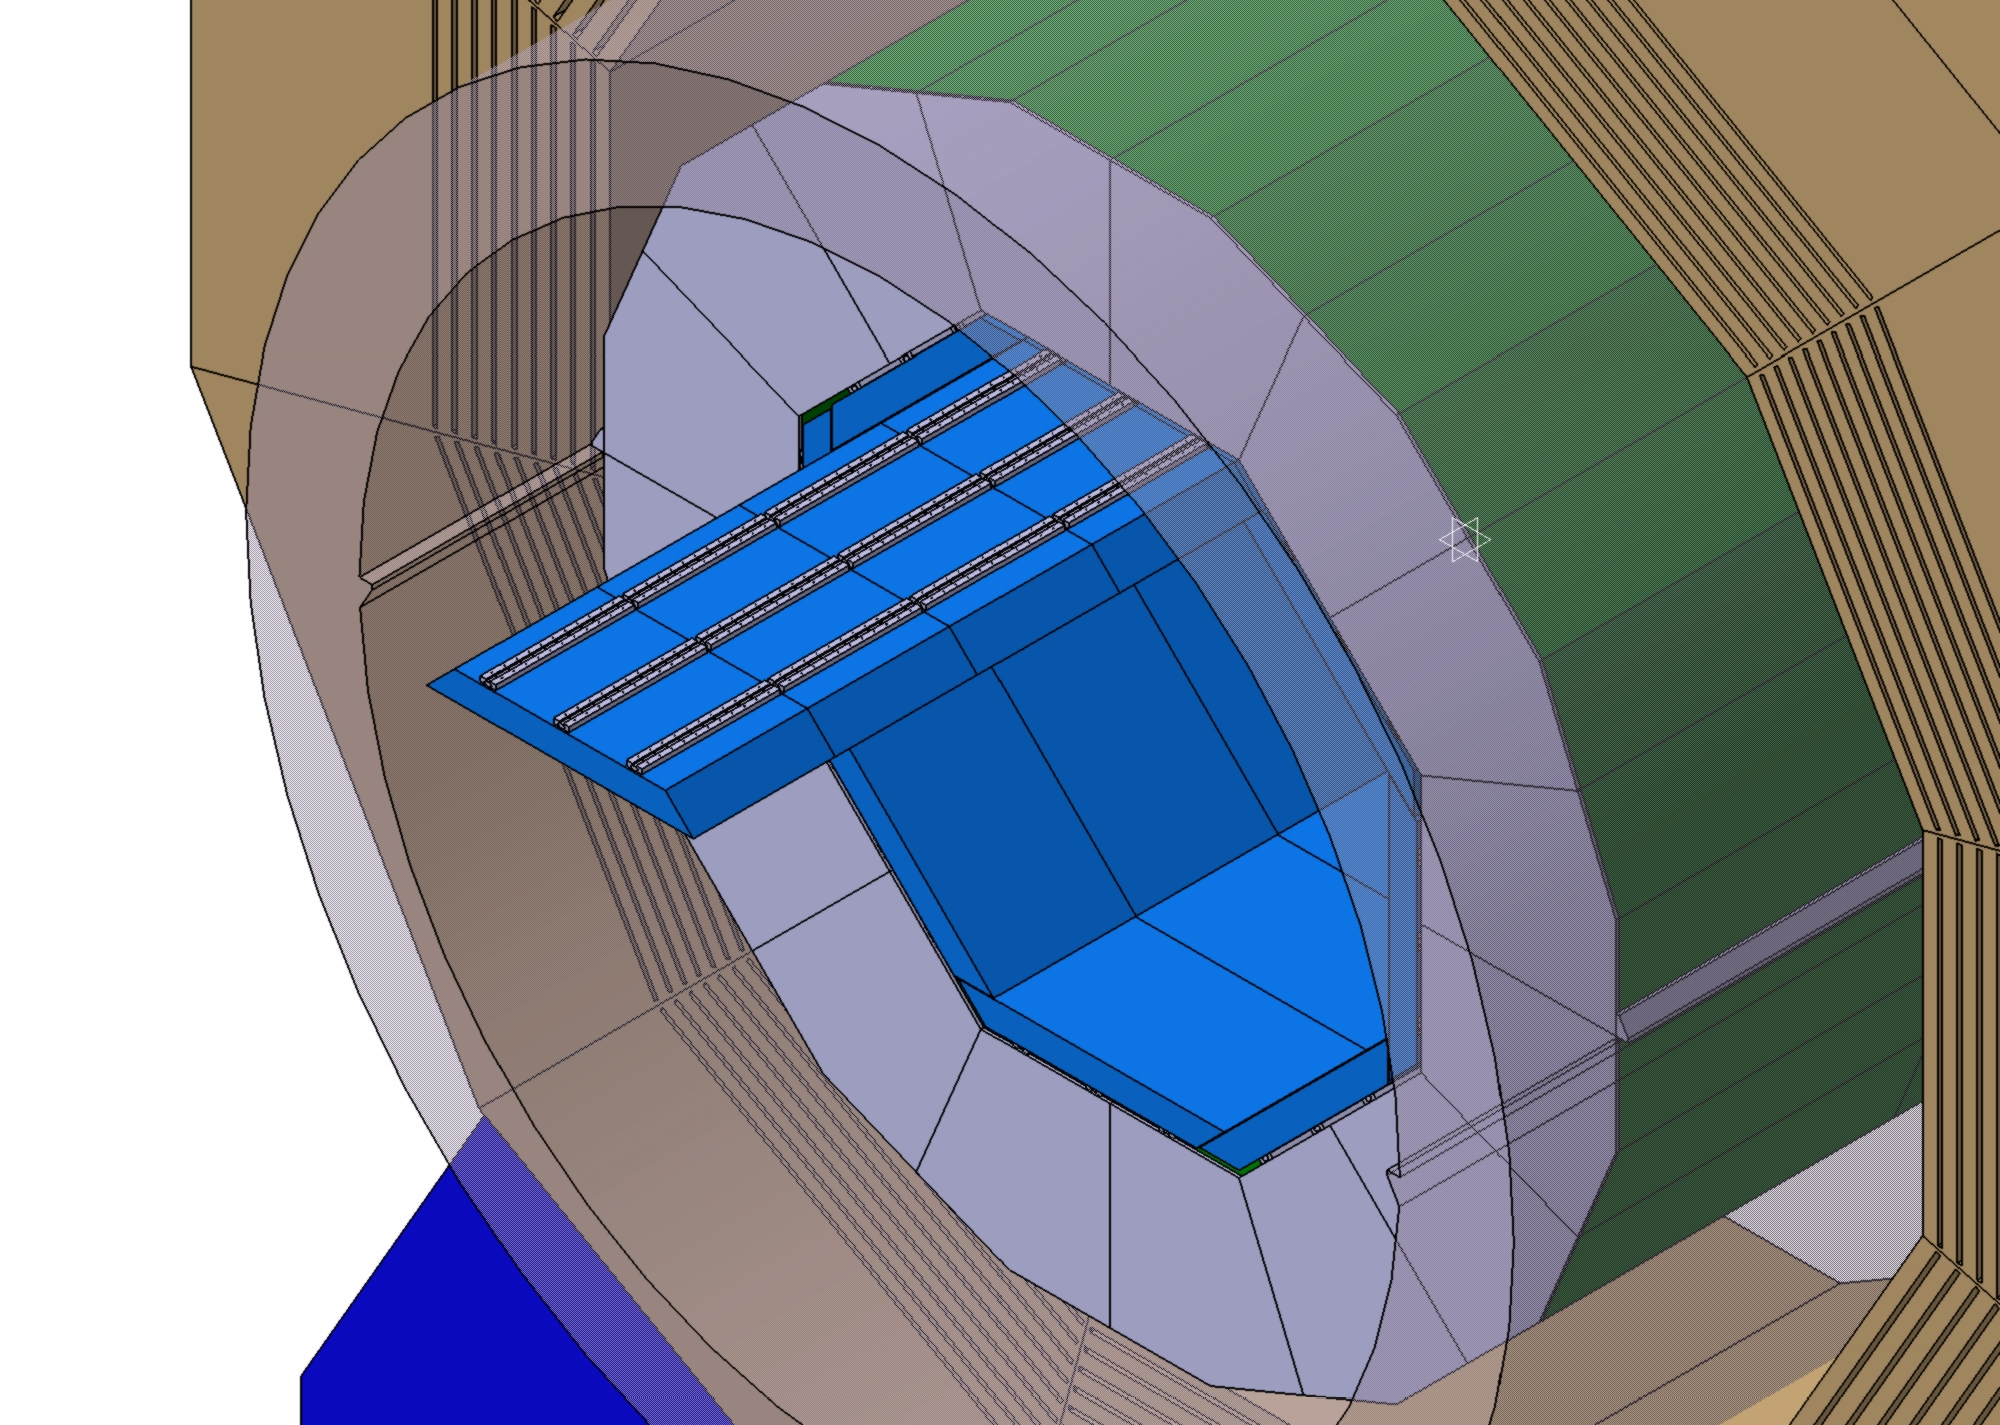
\includegraphics[width=\textwidth]{ILD/ILD_ECAL2}
        \caption{}
        \label{fig:detectorILDECAL2}
    \end{subfigure}
    \begin{subfigure}[b]{0.45\textwidth}
        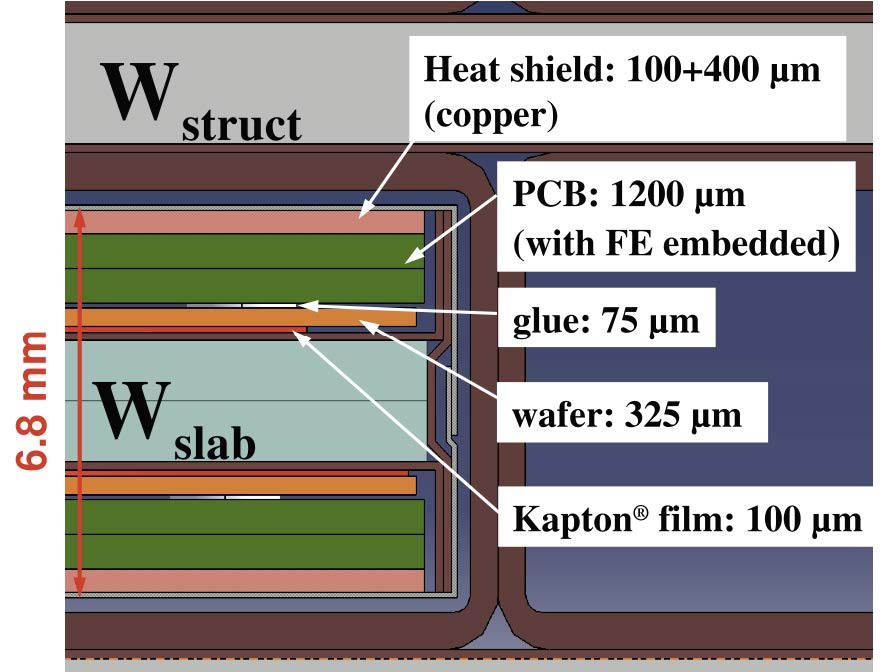
\includegraphics[width=\textwidth]{ILD/ILD_ECAL}
        \caption{}
        \label{fig:detectorILDECAL}
    \end{subfigure}
\caption
{ a) The electromagnetic calorimeter (in blue) within the \ILD detector. b) A cross section through the electromagnetic calorimeter layers. Both plots are  taken from \cite{Behnke:2013lya}.}
 \label{fig:detectorILDECALfull}
\end{figure}

\begin{comment}
The particle flow paradigm has a large impact on the design of the electromagnetic calorimeter system.
A key requirement is the capability of the system to separate overlapping showers from each other.
A calorimeter for particle flow thus needs to be able to do pattern recognition in the shower. The
electromagnetic section has a number of tasks to fulfill. It should be able to reconstruct photons
in the presence of close-by particles. It should be able to reconstruct the detailed properties of the
shower, such as shower shape, starting point and energy to distinguish early starting electromagnetic
showers from hadronic ones. It should be noted that about half of the hadronic showers start inside
the electromagnetic calorimeter. Thus an excellent three-dimensional granularity of the device is of
utmost importance.

The transverse and longitudinal segmentation of both calorimeters has been optimised based on
detailed simulation and test beam data. It has been shown that the granularity must be of the order
of X0 in all three dimensions. This implies that a sampling calorimeter is the best option for both
ECAL and HCAL. For the ECAL the most compact design can be realised with tungsten as absorber
material. For the HCAL iron is chosen as this allows an excellent energy resolution for hadrons at
manageable granularity.
For the ECAL, silicon pad diodes lead to the highest possible compactness (and effective Moli`ere
radius) and exhibit excellent stability of calibration. As an option scintillating strips with silicon
photo-sensor readout are studied, which provide a similar effective segmentation. The two technologies
can be combined in order to reach a cost-performance optimum.

In order to have a better separation of close-by showers in the calorimeter, a system with a
small Moli`ere radius is advantageous. Further help in the separation between electromagnetic and
hadronic showers can come from a large ratio between interaction length and radiation length. A
small radiation length will move the start of the electromagnetic shower earlier in the calorimeter,
while a large interaction length will reduce the fraction of hadronic showers starting in the ECAL.

The particle flow approach requires that the calorimeters are placed inside the magnetic coil,
see Sec. 1.2. This has a major impact on the layout of the detector, and on the cost. Therefore, a
compact calorimeter is preferred in order to minimise the overall physical thickness, which in turn
reduces the size of the coil. For the ECAL tungsten is a good choice for the radiator as it is dense, and
has a large ratio of interaction length to radiation length. The final system layout is a compromise
between performance and cost. The energy resolution scales with OT, where T is the individual
absorber plate thickness, while the cost scales linearly with the surface area of the readout layers. For
ILD a solution with 30 readout layers and a thickness of the ECAL of 24X0 has been chosen as the
baseline. The optimisation of the layout is ongoing.

For a chosen pad size of 5 . 5mm2 silicon pin diodes are a good choice. They can cover large
areas, are reliable and simple to operate, allow for a thin readout layer and can operate in the 3.5 T
strong central magnetic field. While the very thin silicon layers offer excellent performance for the
tracking capabilities of the calorimeter, the energy resolution is somewhat degraded. Here a less
compact device, with a thicker readout layer, will show better performance.

The requirements on granularity, compactness and particle separation lead to the choice of a
sampling calorimeter with tungsten (radiation length X0 = 3.5 mm, Moliere Radius RM = 9 mm and
interaction length = 99 mm) as absorber material. This allows for a compact design with a depth
of roughly 24 X0 within 20 cm and, compared to e.g. lead, a better separation of electromagnetic
showers generated by near-by particles. To achieve an adequate energy resolution, the ECAL is
longitudinally segmented into 30 layers, possibly with varying tungsten thicknesses. In order to
optimise the pattern recognition performance, the active layers (either silicon diodes or scintillator)
are segmented into cells with a lateral size of 5 mm.
\end{comment}

\subsection{Hadronic Calorimeter}



The principal role of the \HCAL is to separate neutral hadron showers from other particles, and to measure (neutral) hadron energies. The \ILD \HCAL  is a sampling calorimeter with steel absorber and scintillator tiles as the active medium. The layout of the \HCAL is  48 longitudinal layers with 3$\times$3\,\uprightMath{{cm}^2} scintillator tiles, using an analogue read out system. The layout of a technological prototype, the "EUDET prototype"  \cite{Collaboration:2011jka} is shown in \Figure{fig:detectorAHCAL}.


For the absorber material, stainless steel is chosen for mechanical and calorimetric reasons. Steel allows a self-supporting structure without auxiliary supports. At the same time, iron has a moderate ratio of hadronic interaction length ($\lambda_I = 17$\,cm) to electromagnetic radiation length ($X_0=1.8$\,cm), which allows a fine longitudinal sampling in $X_0$ with a reasonable number of layers in a given total hadronic absorption length.  The longitudinal system, including the \ECAL, provides about 6 interaction lengths, which is sufficient to contain the hadronic showers.


The scintillator tiles provide both energy and position measurement. The transverse segmentation, chosen by optimisation studies \cite{Thomson:2009rp} is about 3$\times$3\,\uprightMath{cm^2}. This level of segmentation is sufficient to meet the requirement of the particle flow \cite{Behnke:2013lya}.

%  The requirement of three dimensional granularity in transverse and longitudinal directions is satisfied by a sampling calorimeter with steel absorber and scintillator tiles as active medium.



\begin{figure}[tbph]
\centering
    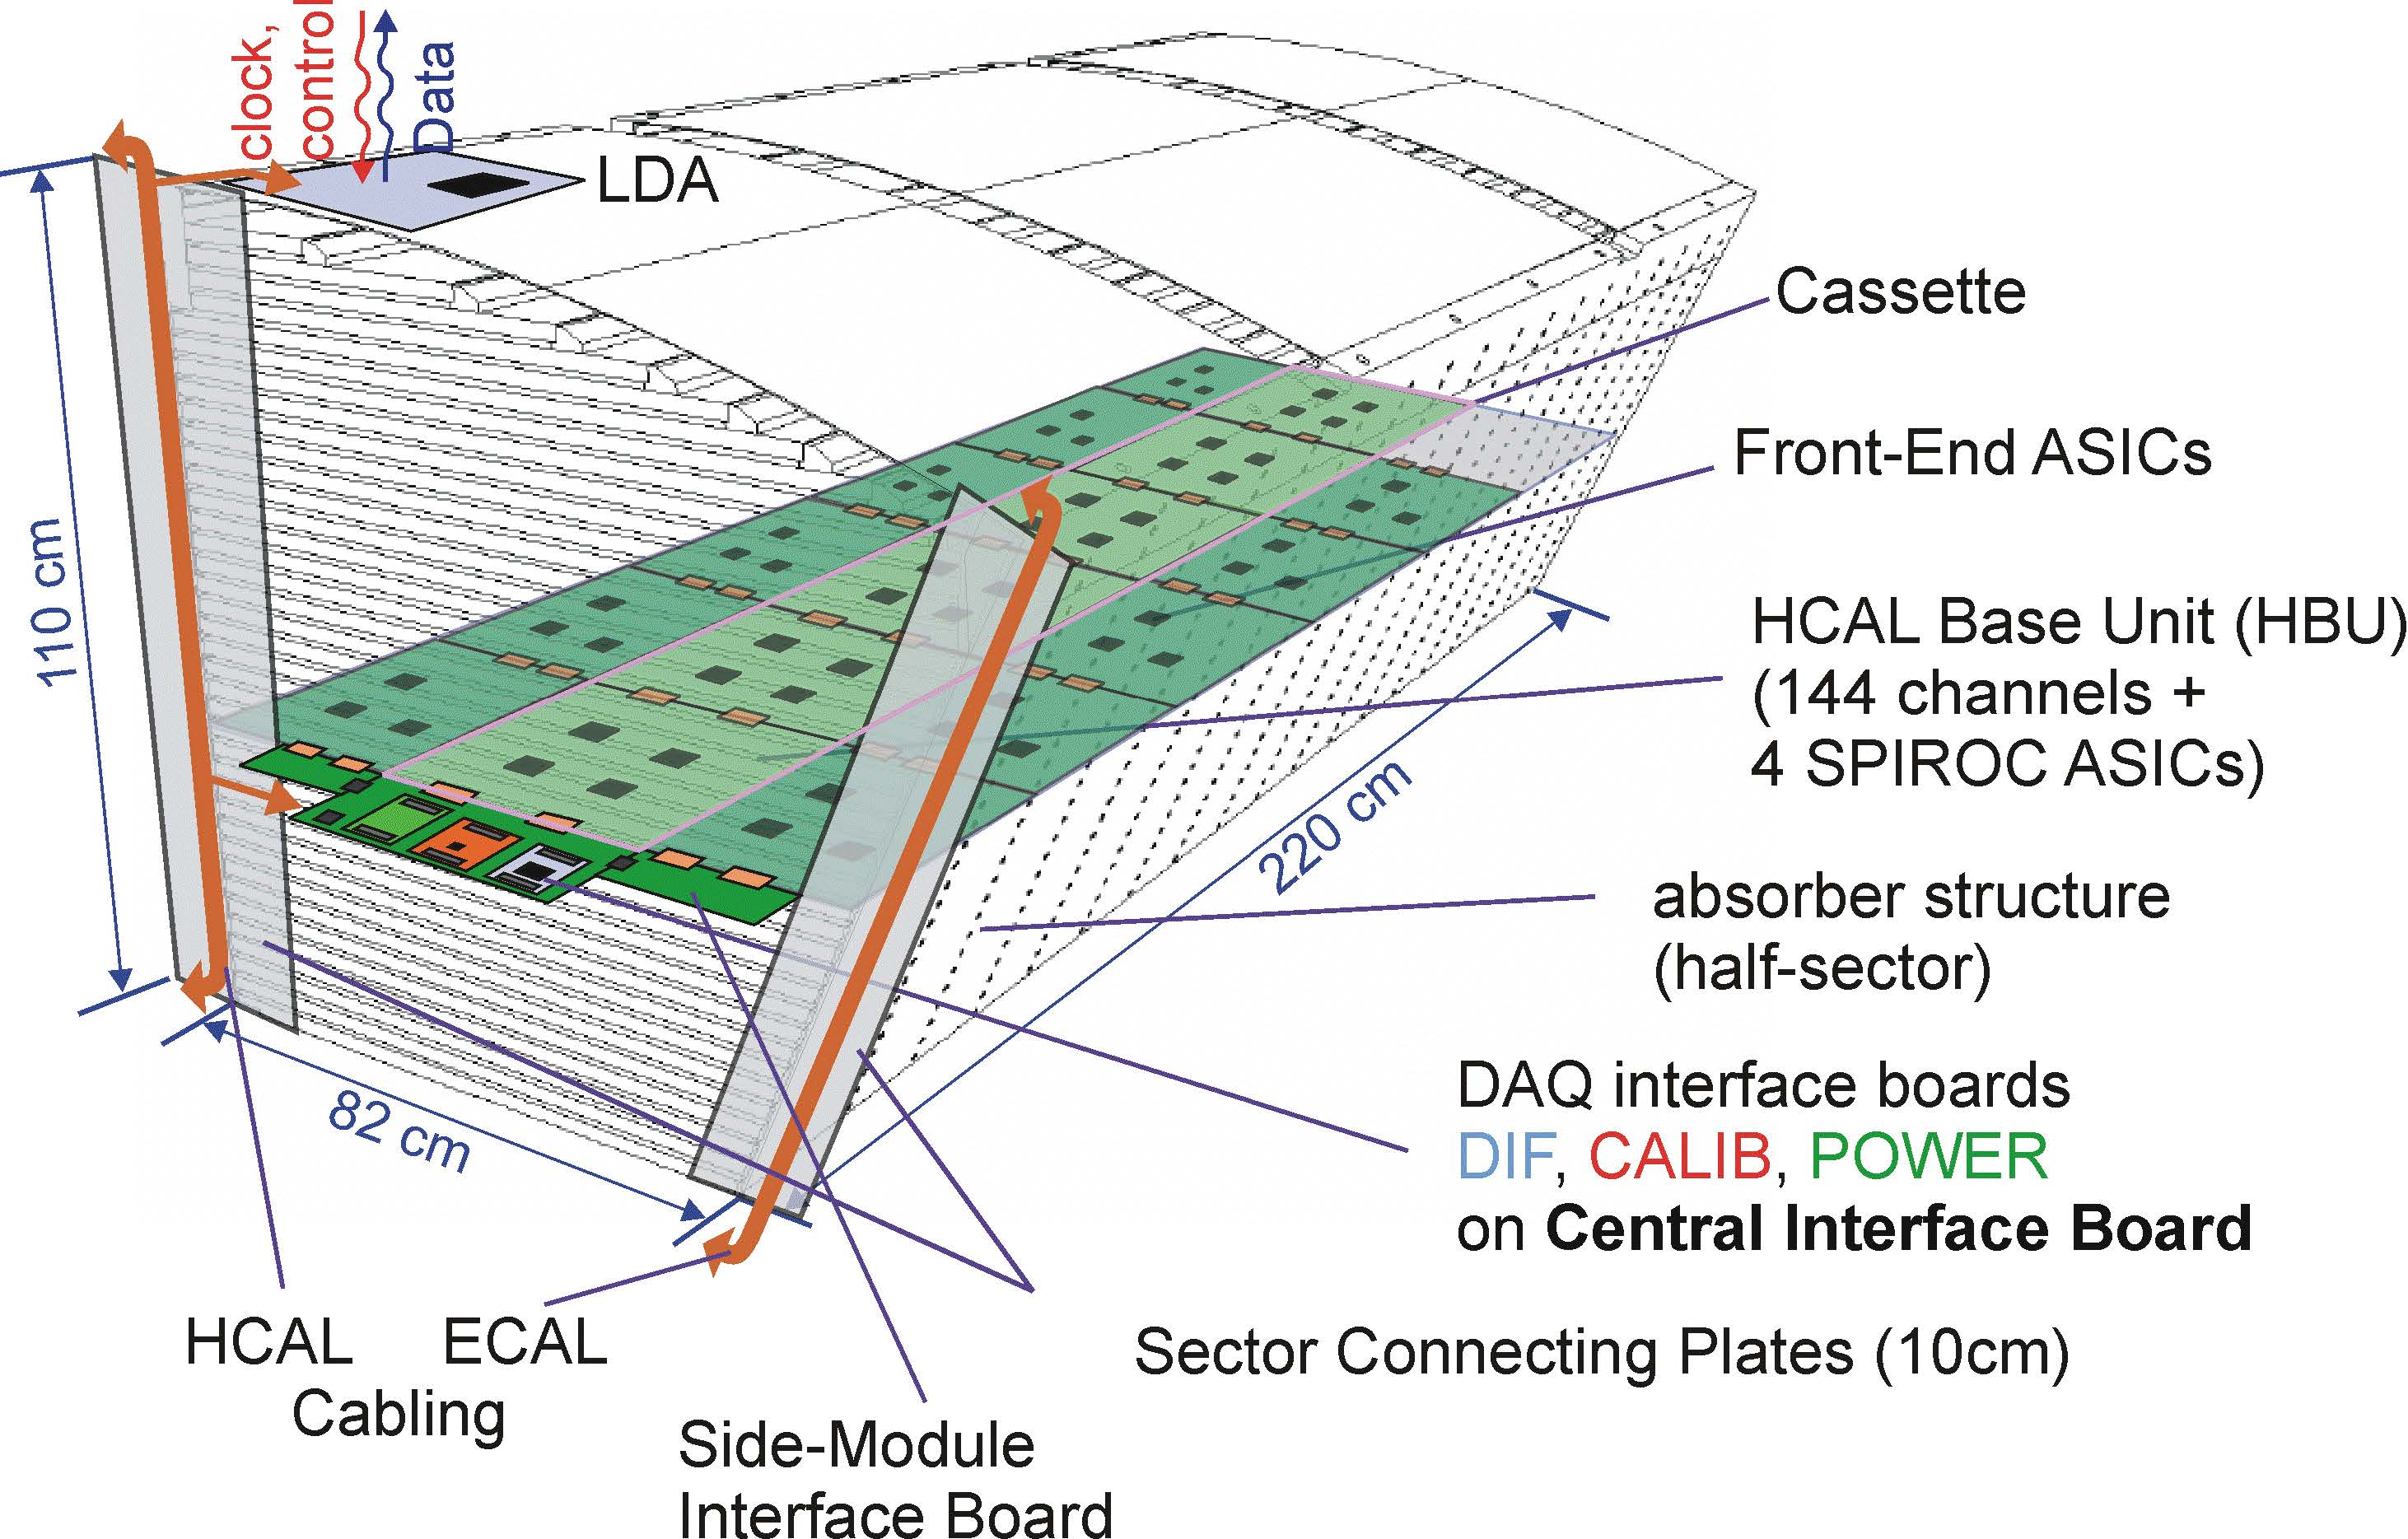
\includegraphics[width=0.45\textwidth]{ILD/ILD_AHCAL}

\caption
{The schematic view of a CALICE analogue HCAL technological prototype module, taken from \cite{Behnke:2013lya}.}
    \label{fig:detectorAHCAL}
\end{figure}


\begin{comment}
The role of the HCAL is to separate the deposits of charged and neutral hadrons and to precisely
measure the energy of the neutrals. Their contribution to the jet energy, around 10% on average,
fluctuates over a wide range from event to event, and the accuracy of the measurement is the
dominant contribution to the particle flow resolution for jet energies up to about 100 GeV. For higher
energies, the performance is dominated by confusion, and both topological pattern recognition and
energy information are important for correct track cluster assignment.


This is followed by a highly segmented hadronic calorimeter (HCAL) with up to 48 longitudinal
samples and small transverse cell size. Two options are considered, both based on a Steel-absorber
structure. One option uses scintillator tiles of 3 . 3 cm2, which are read out with an analogue
system. The second uses a gas-based readout which allows a 1.1 cm2 cell geometry with a binary or semi-digital readout of each cell.


The HCAL is optimized to measure neutral hadrons
well and thus has to provide the topological resolution power for separating them from the showers of
the much more abundant charged hadrons which must be matched with tracks.


The transverse and longitudinal segmentation of both calorimeters has been optimised based on
detailed simulation and test beam data. It has been shown that the granularity must be of the order
of X0 in all three dimensions. This implies that a sampling calorimeter is the best option for both
ECAL and HCAL. For the ECAL the most compact design can be realised with tungsten as absorber
material. For the HCAL iron is chosen as this allows an excellent energy resolution for hadrons at
manageable granularity.



The role of the HCAL is to separate the deposits of charged and neutral hadrons and to precisely
measure the energy of the neutrals. Their contribution to the jet energy, around 10% on average,
fluctuates over a wide range from event to event, and the accuracy of the measurement is the
dominant contribution to the particle flow resolution for jet energies up to about 100 GeV. For higher
energies, the performance is dominated by confusion, and both topological pattern recognition and
energy information are important for correct track cluster assignment.




The HCAL is conceived as a sampling calorimeter with steel absorber and scintillator tiles
(analogue HCAL) or gaseous devices (semi-digital HCAL) as active medium. Due to the rigidity of
stainless steel, a self-supporting structure without auxiliary supports (dead regions) can be realised.
Moreover, in contrast to heavier materials, iron with its moderate ratio of hadronic interaction length
(.I = 17 cm) to electromagnetic radiation length (X0 = 1.8 cm) allows a fine longitudinal sampling
in terms of X0 with a reasonable number of layers in a given total hadronic absorption length, thus
keeping the detector volume and readout channel count at an acceptable level. This fine sampling is
beneficial both for the measurement of the sizeable electromagnetic energy part in hadronic showers
and for the topological resolution of shower substructure, needed for particle separation and weighting.
Two baseline technology options have been developed, the scintillator-tile based AHCAL and the
Glass Resistive Plate Chamber (GRPC) based SDHCAL.
\end{comment}

\subsection{Solenoid, Yoke and Muon system}

A large superconducting solenoid, outside the calorimeters, produces a nominal  3.5\,T magnetic field. \FIGURE{fig:detectorILDSolenoid} shows the cross section of the \ILD magnet.

\begin{figure}[tbph]
\centering
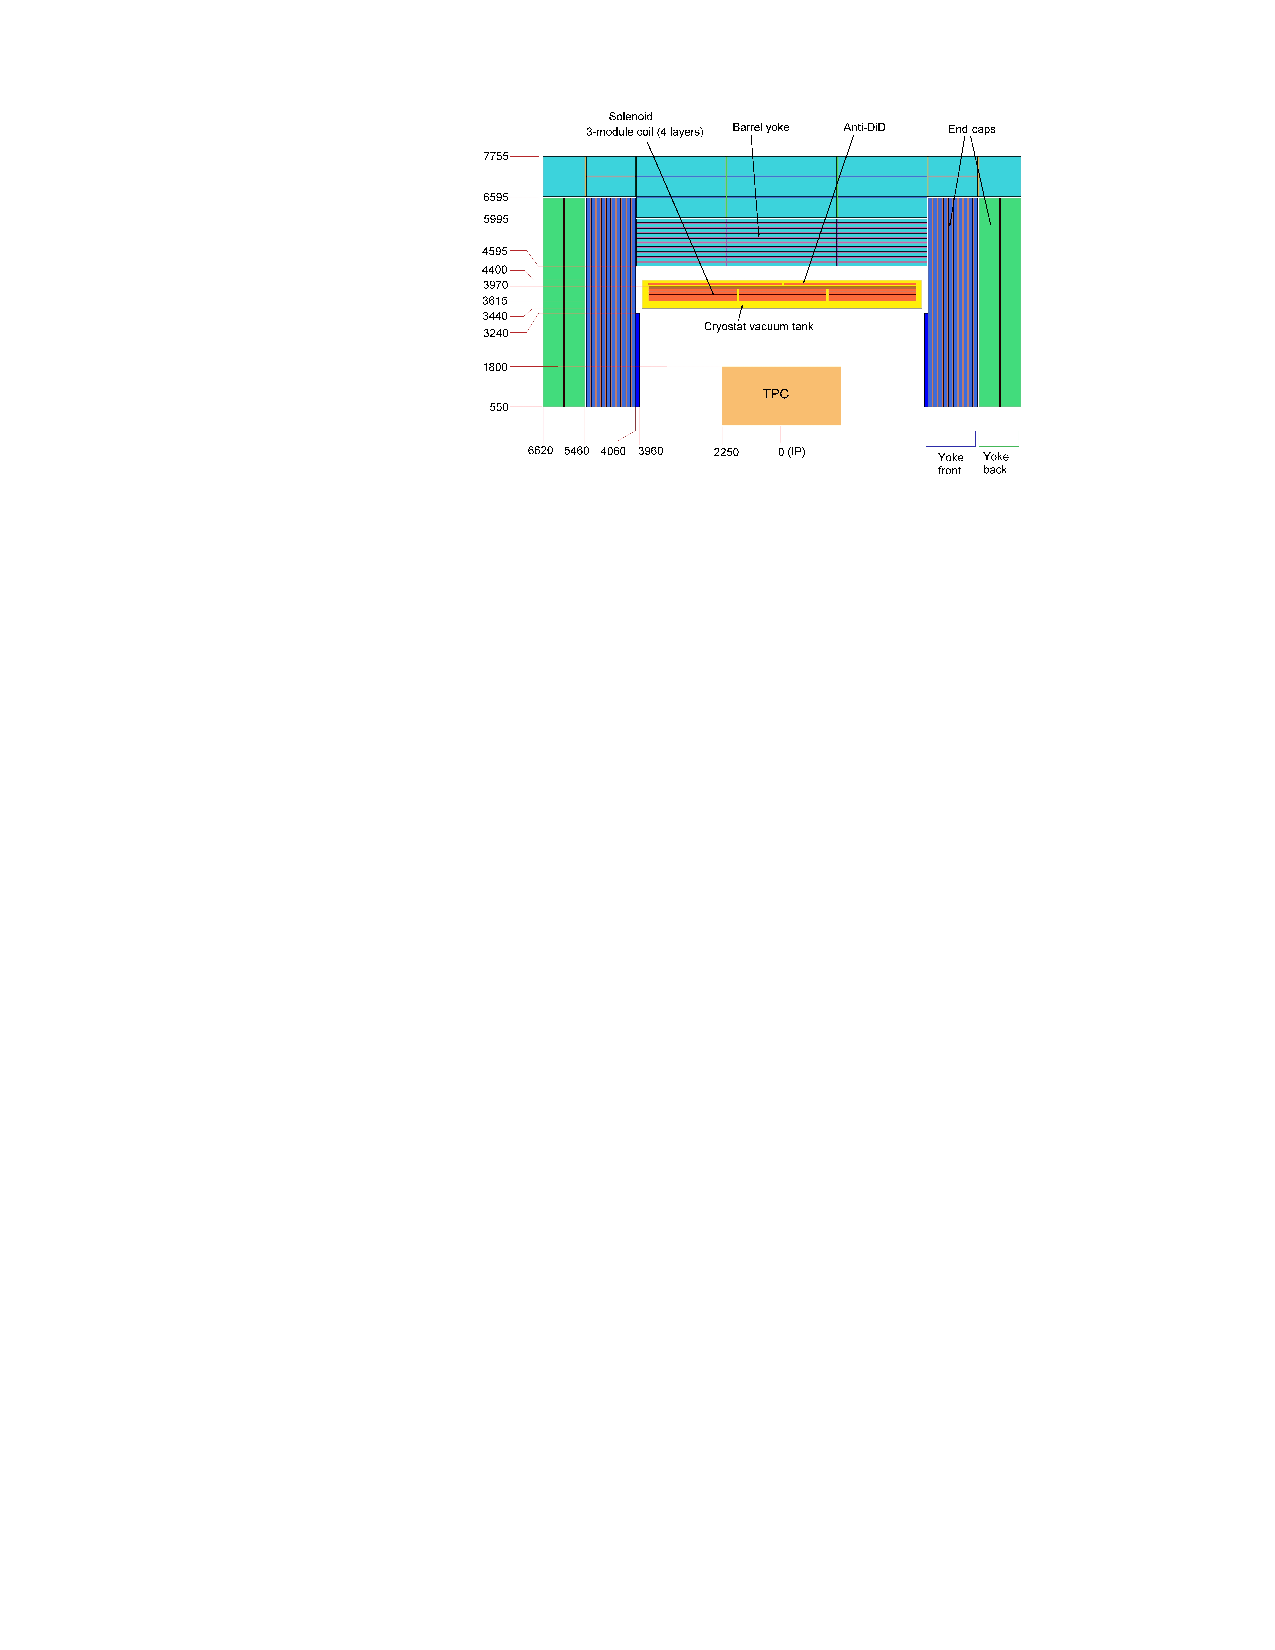
\includegraphics[width=0.65\textwidth]{ILD/ILD_solenoid}
\caption
{The \ILD magnet cross section. Dimensions are in mm. Figure is taken from \cite{Behnke:2013lya}.}
\label{fig:detectorILDSolenoid}
\end{figure}


The iron  yoke returns the magnetic flux. The yoke is designed to ensure that the maximum magnetic field at 15\,m radial distance from the detector is 50 Gauss to ensure safety \cite{Parker:21354}. 

The iron yoke is also instrumented with scintillator strips as active layers to act as a muon detector.  A highly efficient muon detector is provided by the 3$\times$3\,\uprightMath{{cm}^2} scintillator tiles. The layout of the muon detector is shown in \Figure{fig:detectorILDMuon}.

The first layer of the muon detector, also acting as a tail catcher calorimeter, catches the energy leakage from the \HCAL and the \ECAL. It has been shown that a 10\% improvement of single particle energy resolution is possible with the tail catcher \cite{CALICE:2012aa}.

%An iron yoke is instrumented with scintillator strips as active layers. The iron  yoke returns the magnetic flux, and also acts as a muon detector and hadronic shower tail catcher calorimeter at the same time. The layout of the muon detector is shown in \Figure{fig:detectorILDMuon}. A highly efficient muon detector is provided by the 3$\times$3\,\uprightMath{{cm}^2} scintillator tiles.  The first layer of the muon detector, also acting as a tail catcher calorimeter, catches the energy leakage from the \HCAL and the \ECAL. It has been shown that a 10\% improvement of single particle energy resolution is possible with the tail catcher \cite{CALICE:2012aa}.





\begin{figure}[tbph]
\centering
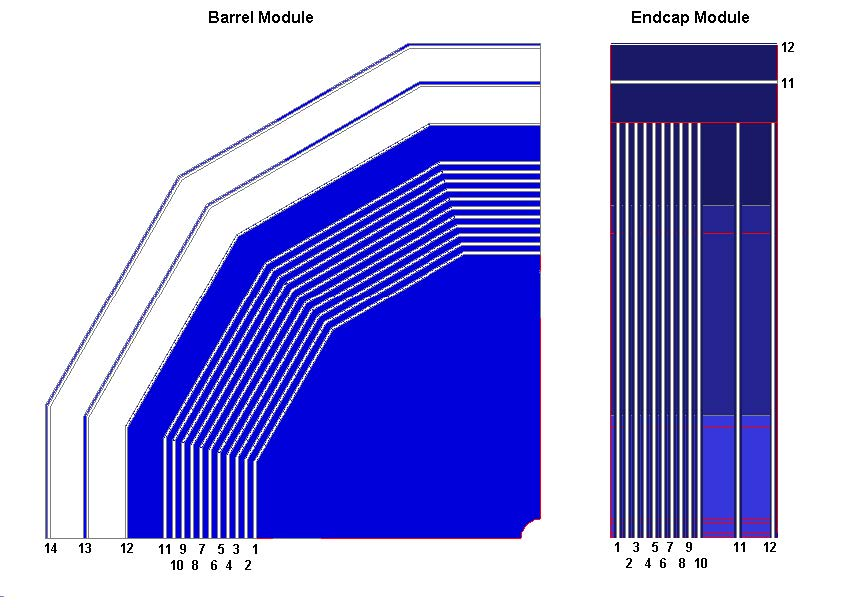
\includegraphics[width=0.65\textwidth]{ILD/ILD_Muon}
\caption
{Sensitive layers of the \ILD muon system, taken from \cite{Behnke:2013lya}.}
\label{fig:detectorILDMuon}
\end{figure}

\begin{comment}
the iron Yoke has been instrumented with scintillator based active layers. At the
moment tiles with 3 . 3 cm2 granularity are used, for muon detection and serving as a tail
catcher for the HCAL; this is different than the detector baseline which uses 3 cm wide and 1
m long strips;

During beam operation the IR hall has to be accessible due to the push-pull concept. Since all
activities in a high magnetic field are very cumbersome and potentially dangerous, a field limit of 50 G
at 15 m radial distance from the beam line was agreed upon [354]. Two- and three-dimensional FEM
field calculations were done using the CST EM Studio programme, varying the thickness and geometry
of the iron in the barrel and end-caps until the goal of less than 50 G at 15 m radial distance was
achieved.



An iron yoke, instrumented with scintillator strips or resistive plate chambers (RPCs), returns
the magnetic flux of the solenoid, and, at the same time, serves as a muon filter, muon detector and
tail catcher calorimeter

A stable, highly efficient muon identification system with excellent hadron rejection is an important
requirement to meet the physics goals of the ILD detector. The ILD muon system provides a number
of measurement stations outside the solenoid coil, which supplement the measurements taken with
the calorimeter system and the tracker. It is used to identify the muons and to act as a tail catcher, to
recover energy which is leaking out of the back of the calorimeter. However, the barrel part location
behind the coil limits its role to fairly high momentum particles.
The muon system/ tail catcher instruments the iron return yoke in the barrel and in the forward
region. The yoke barrel part is equipped with one sensitive layer in front of the iron yoke, 10 layers
spaced 14 cm apart, followed by three sensitive layers spaced by 60 cm apart. The forward part of the
yoke is equipped with 10 layers spaced by 14 cm, followed by two sensitive layers spaced by 60 cm.
The overall layout of the muon system/ tail catcher is shown in Figure

The first layers of the muon system serve as a tail catcher, measuring the energy which leaks through
the end of the calorimeter system. Figure III-4.5 shows the effect of an ideal tail catcher (no dead
material between the calorimeter and the tail catcher) and the realistic scenario at ILD, with two
interaction lengths of material in front of the tail catcher, as a function of the total depth of the
calorimeter system. For 6 ., the value for the ILD calorimeter system, a roughly 10% improvement is
possible with the tail catcher [348].
A prototype of the muon system/tail catcher was successfully tested during the 2007-2012
CALICE test beam campaign with ECAL and analogue HCAL. A tail catcher was placed behind the
HCAL instrumented with scintillator strips and readout with SiPMs [348]. Results from the tests
show that the proposed system delivers the anticipated performance and thus validates the technology
needed to built a muon system for ILD.
\end{comment}

\subsection{Very Forward Calorimeters}

The detectors in the forward region provide luminosity measurements and forward coverage of calorimeters. A system of precision and radiation resistent calorimeters is required. \FIGURE{fig:detectorILDForward} shows the forward calorimeters of the \ILD. 

The luminosity calorimeter (\LumiCAL) counts  Bhabha scattering to measure the luminosity to precision of $10^{-3}$ at a centre-of-mass energy of  500\,GeV \cite{1748-0221-3-10-P10004}. The beam calorimeter (\BeamCAL), which is hit by many beamstrahlung pairs after each bunch crossing, extends the forward coverage. The \BeamCAL also provides a measurement of the bunch-by-bunch luminosity. An additional hadron calorimeter in the forward region, \LHCAL,  extends the angular coverage of the \HCAL to that of the \LumiCAL. 


The calorimeters in the  forward region also provides enough information for high-energy electron tagging \cite{sailer2012radiation}, which aids event reconstruction at a high centre-of-mass energy. \TABLE{tab:detectorForwardILDvsCLICILD} lists the key parameters of the \LumiCAL and the \BeamCAL in the \ILD.


\begin{figure}[tbph]
\centering
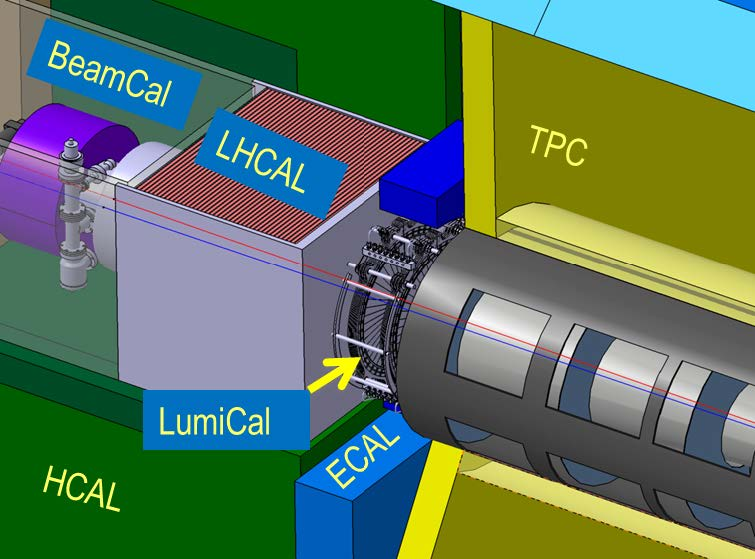
\includegraphics[width=0.45\textwidth]{ILD/ILD_forward}
\caption[The forward calorimeters of the \ILD.]
{The  calorimeter in the forward region of the \ILD, taken from \cite{Behnke:2013lya}. The \LumiCAL, the \BeamCAL, and the \LHCAL are the luminosity calorimeter, the beam calorimeter, and the forward hadronic calorimeter, respectively.}
\label{fig:detectorILDForward}
\end{figure}

\begin{comment}

At very forward angles, below the coverage provided by the ECAL and the HCAL, a system of
high precision and radiation hard calorimetric detectors (LumiCAL, BeamCAL, LHCAL) is foreseen.
These extend the calorimetric coverage to almost 4fi, measure the luminosity, and monitor the quality
of the colliding beams

Two special calorimeters are foreseen in the very forward regions of the detector [324], denoted
hereafter as LumiCal and BeamCal. LumiCal will measure the luminosity with a precision of better
than 10��3 at 500 GeV centre-of-mass energy1, and BeamCal will perform a bunch-by-bunch estimate
of the luminosity and, supplemented by a pair monitor, assist beam tuning when included in a fast
feedback system [325]. Both calorimeters extend the detector coverage to low polar angles, important
e.g. for new particle searches with missing energy signature [326]. The additional low angle hadron
calorimeter LHCAL extends the coverage of the hadron calorimeter to the polar angle range of
LumiCal. A sketch of the design is shown in Figure III-3.24.
LumiCal is positioned in a circular hole of the end-cap electromagnetic calorimeter ECAL.
BeamCal is placed just in front of the final focus quadrupole. LumiCal covers polar angles between
31 and 77 mrad and BeamCal between 5 and 40 mrad.
Due to the high occupancy originating from beamstrahlung and two-photon processes, both
calorimeters need a fast readout. In addition, the lower polar angle range of BeamCal is exposed to a
large flux of low energy electrons, resulting in radiation depositions up to one MGy per year. Hence,
radiation hard sensors are needed.

\end{comment}


%This section will describe sub-systems from small to large radius.


\begin{table}[htbp]
\centering
\smallskip
\begin{tabular}{l l r  r }
\hline
\hline
 & &  \ILD & \CLICILD \\
\hline
\multirow{4}{*}{\LumiCAL} & Geometrical acceptance  & 31 - 77\,mrad & 38 - 110\,mrad \\
& Fiducial acceptance& 41 - 67\,mrad & 44 - 80\,mrad \\
& z (start) & 2450\,mm & 2654\,mm \\
& Number of layers (W + Si) & 30 & 40 \\
\hline
\multirow{4}{*}{\BeamCAL} & Geometrical acceptance & 5 - 40\,mrad & 10 - 40\,mrad \\
& z (start)  & 3600\,mm & 3281\,mm \\
& Number of layers (W + sensor) & 30 & 40 \\
& Graphite layer thickness  & 100\,mm & 100\,mm \\
\hline
\hline
\end{tabular}
\caption[Comparison of the \LumiCAL and the \BeamCAL at the \ILD and the \CLICILD .]%
{Comparison of the key parameters for the \LumiCAL and the \BeamCAL at the \ILD and the \CLICILD detector concepts. The table is adapted from \cite{Linssen:2012hp}. }
\label{tab:detectorForwardILDvsCLICILD}
\end{table}

\begin{comment}
The International Large Detector (ILD) is a concept for a detector at the International Linear Collider,
ILC [198]. In a slightly modified version, it has also been proposed for the CLIC linear collider [199].
The ILD detector concept has been optimised with a clear view on precision. In recent years
the concept of particle flow has been shown to deliver the best possible overall event reconstruction.
Particle flow implies that all particles in an event, charged and neutral, are individually reconstructed.
This requirement has a large impact on the design of the detector, and has played a central role in
the optimisation of the system. Superb tracking capabilities and outstanding detection of secondary
vertices are other important aspects. Care has been taken to design a hermetic detector, both in
terms of solid-angle coverage, but also in terms of avoiding cracks and non-uniformities in response.
The overall detector system has undergone a vigorous optimisation procedure based on extensive
simulation studies both of the performance of the subsystems, and on studies of the physics reach
of the detector. Simulations are accompanied by an extensive testing programme of components and
prototypes in laboratory and test-beam experiments.
Figure III-1.1
View of the ILD detector
concept.
The ILD detector concept has been described in a number of documents in the past. Most
recently the letter of intent [198] gave a fairly in depth description of the ILD concept. The ILD
concept is based on the earlier GLD and LDC detector concepts [200, 201, 202]. Since the publication
of the letter of intent, major progress has been made in the maturity of the technologies proposed for
ILD, and their integration into a coherent detector concept
\end{comment}


\section{Detector optimisation}


%\section{\CLIC versus the \ILC}


%The two main differences between \CLIC and the \ILC are the high centre-of-mass energy and the high bunch charge density at \CLIC, which leads to significant beam related backgrounds.  At \CLIC, within a bunch train, there is 0.5\,ns between bunch crossings.  There are two main sources of beam induced background at \CLIC colliding environment: incoherent electron pairs from  photon (real or virtual) interactions with individual particles of the other beam, and interactions of two photons from the colliding beams. These differences leads to a modification in the detector design and the reconstruction software for \CLIC.

Detector optimisation studies were performed to choose the optimal parameters for the \ILD sub-detectors\cite{Behnke:2013lya}. Here the optimisation studies for the \ECAL and the \HCAL are presented.

\subsection{Electromagnetic Calorimeter optimisation}

The metric for optimisation is the jet energy resolution, which defined as the \rms divided by the mean for the smallest width of distribution that contains 90\% of entries, using \eeZuds, at barrel region. The angular cut is to avoid the barrel/endcap overlap region. The light quark decay of the \Zprime is used  to avoid the complication of  missing momentum from semi-leptonic decay of heavy quarks. Using 90\% of the entries is robust and focuses on the Gaussian part of the distribution.
%The total jet energy is determined for \sqrtS= 91, 200, 360 and 500\,GeV.

The optimisation of the \ILD \ECAL design was performed as a function of the number of longitudinal layers, whilst keeping other geometry constant.  \FIGURE{fig:detectorILDECALjer} shows the jet energy resolution for a single jet as a function of the number of longitudinal layer, for four different jet energies. For a 45\,GeV jet, a degradation  of 10\% in the jet energy resolution is observed when the number of layers decreases from 30 to 20. The degradation in the jet energy resolution is significant for number of layers fewer than 20, although the impact is smaller for high energy jets. Therefore, 30 longitudinal layers is chosen for the \ECAL.

\begin{figure}[tbph]
\centering
    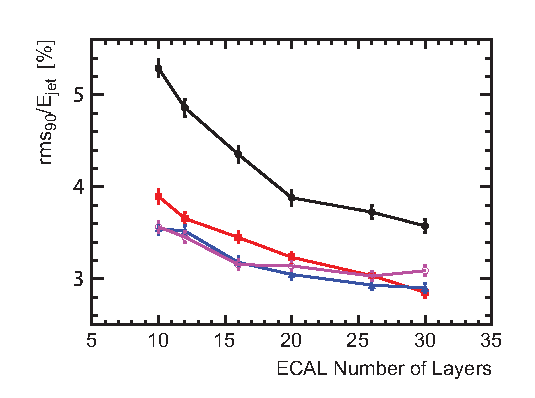
\includegraphics[width=0.55\textwidth]{ILD/ILD_ECAL_layer}
\caption
{The single jet energy resolution as a function of the number of longitudinal \ECAL layers, with  different  total jet energy using \eeZuds, at barrel region, adapted from \cite{Behnke:2013lya}.}
    \label{fig:detectorILDECALjer}
\end{figure}

The \ILD \ECAL design was optimised as a function of the transverse cell sizes, whilst keeping other geometry constant. \FIGURE{fig:detectorILDECALtrans} shows the jet energy resolution for a single jet, plotted as a function of transverse scintillator cell sizes for four different jet energies. The 10$\times$10\,\uprightMath{mm^2} cell size is needed to meet the jet energy requirement of $\sigma_E / E <$3.8\% for the jet energies relevant at \rootS{1}, with 5$\times$5\,\uprightMath{mm^2} cell size being preferable.


\begin{figure}[tbph]
\centering
    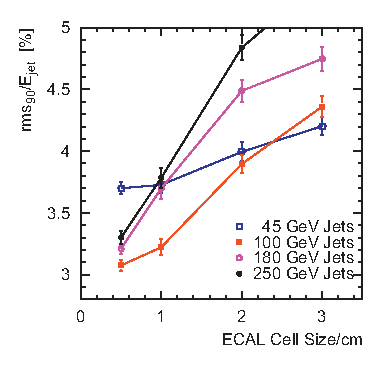
\includegraphics[width=0.45\textwidth]{ILD/ILD_ECAL_cell}
\caption
{The single jet energy resolution as a function of the  \ECAL transverse cell sizes, with  different  total jet energy using \eeZuds, at barrel region, adapted from \cite{Thomson:2009rp}.}
    \label{fig:detectorILDECALtrans}
\end{figure}


\subsection{Hadronic calorimeter optimisation}

For the \ILD \HCAL design, the transverse cell sizes has been optimised using  the  jet energy resolution as the metric. The jet energy resolutions as a function of \HCAL scintillator square cell sizes for foure different jet energies are shown in \Figure{fig:detectorHCALoptimise}. There is no substantial gain in the jet energy resolution for cell sizes below 3\,cm. However, the jet energy resolution degrades for cell sizes above 3\,cm. Hence 3$\times$3\,\uprightMath{cm^2} scintillator cell size is chosen for the \HCAL design.


\begin{figure}[tbph]
\centering
    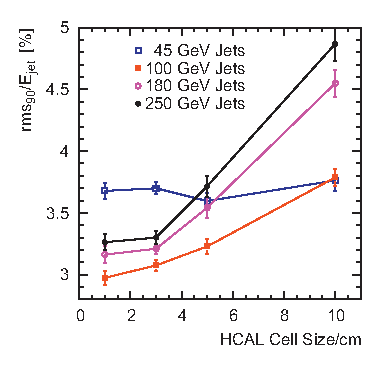
\includegraphics[width=0.45\textwidth]{ILD/ILD_HCAL_cell}
\caption
{The single jet energy resolution as a function of the hadronic calorimeter scintillator cell sizes, with different total jet energy using \eeZuds, at barrel region, adapted from \cite{Behnke:2013lya}.}
    \label{fig:detectorHCALoptimise}
\end{figure}

\begin{comment}
\section{Detector performance}


\subsection{Vertex detector performance}
For the \ILD vertex detector, \Figure{fig:detectorVertexResolution} shows the impact parameter resolution as a function of the particle momentum for  two different particle production angles from test beam results \cite{Behnke:2013lya}. The curves with long dashes show the performance goal. The figure shows that the desired impact parameter resolution is achievable.



\begin{figure}[tbph]
\centering
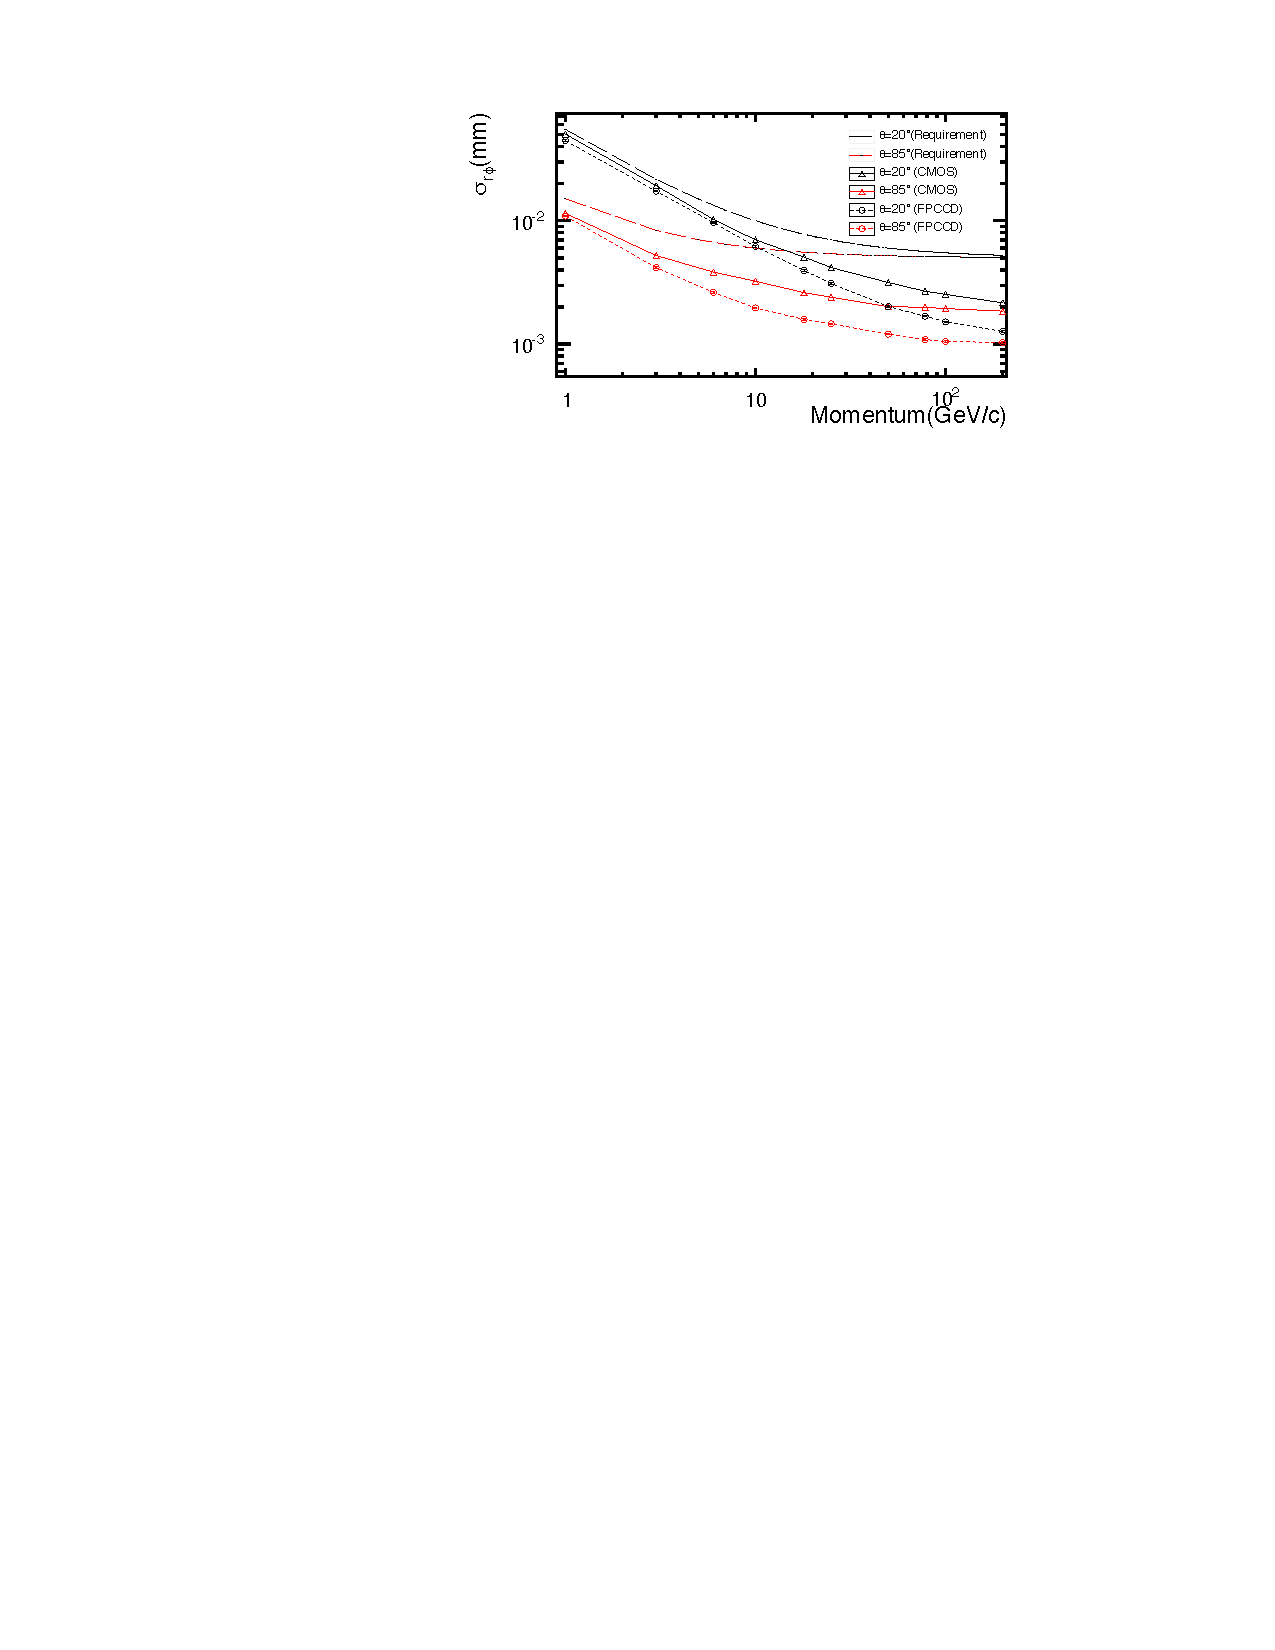
\includegraphics[width=0.55\textwidth]{ILD/vertexResolution}
\caption
{Impact parameter resolution of the \ILD vertex detector for two different particle production angles (20\degree and 85\degree), assuming the baseline point resolution given in \Table{tab:detectorVertex} for CMOS option (solid line), and the FPCCD option (dotted line). The curves with long dashes show the performance goal. The figure is taken from \cite{Behnke:2013lya}.}
\label{fig:detectorVertexResolution}
\end{figure}

\subsection{Particle flow performance}

\FIGURE{fig:detectorJERangle} shows the jet energy resolution as a function of the polar angle of the \Zprime, using \eeZuds, at barrel region of the detector. There is a degradation in the energy resolution for the barrel/endcap overlap region, corresponding to \uprightMath{0.7 < \absOf{\cos \theta} < 0.8}. A small degradation in the performance at \uprightMath{\cos\theta \approx 0} is seen because of the \TPC central membrane and gaps between sections of the \HCAL in the \ILD detector simulation.

\begin{figure}[tbph]
\centering
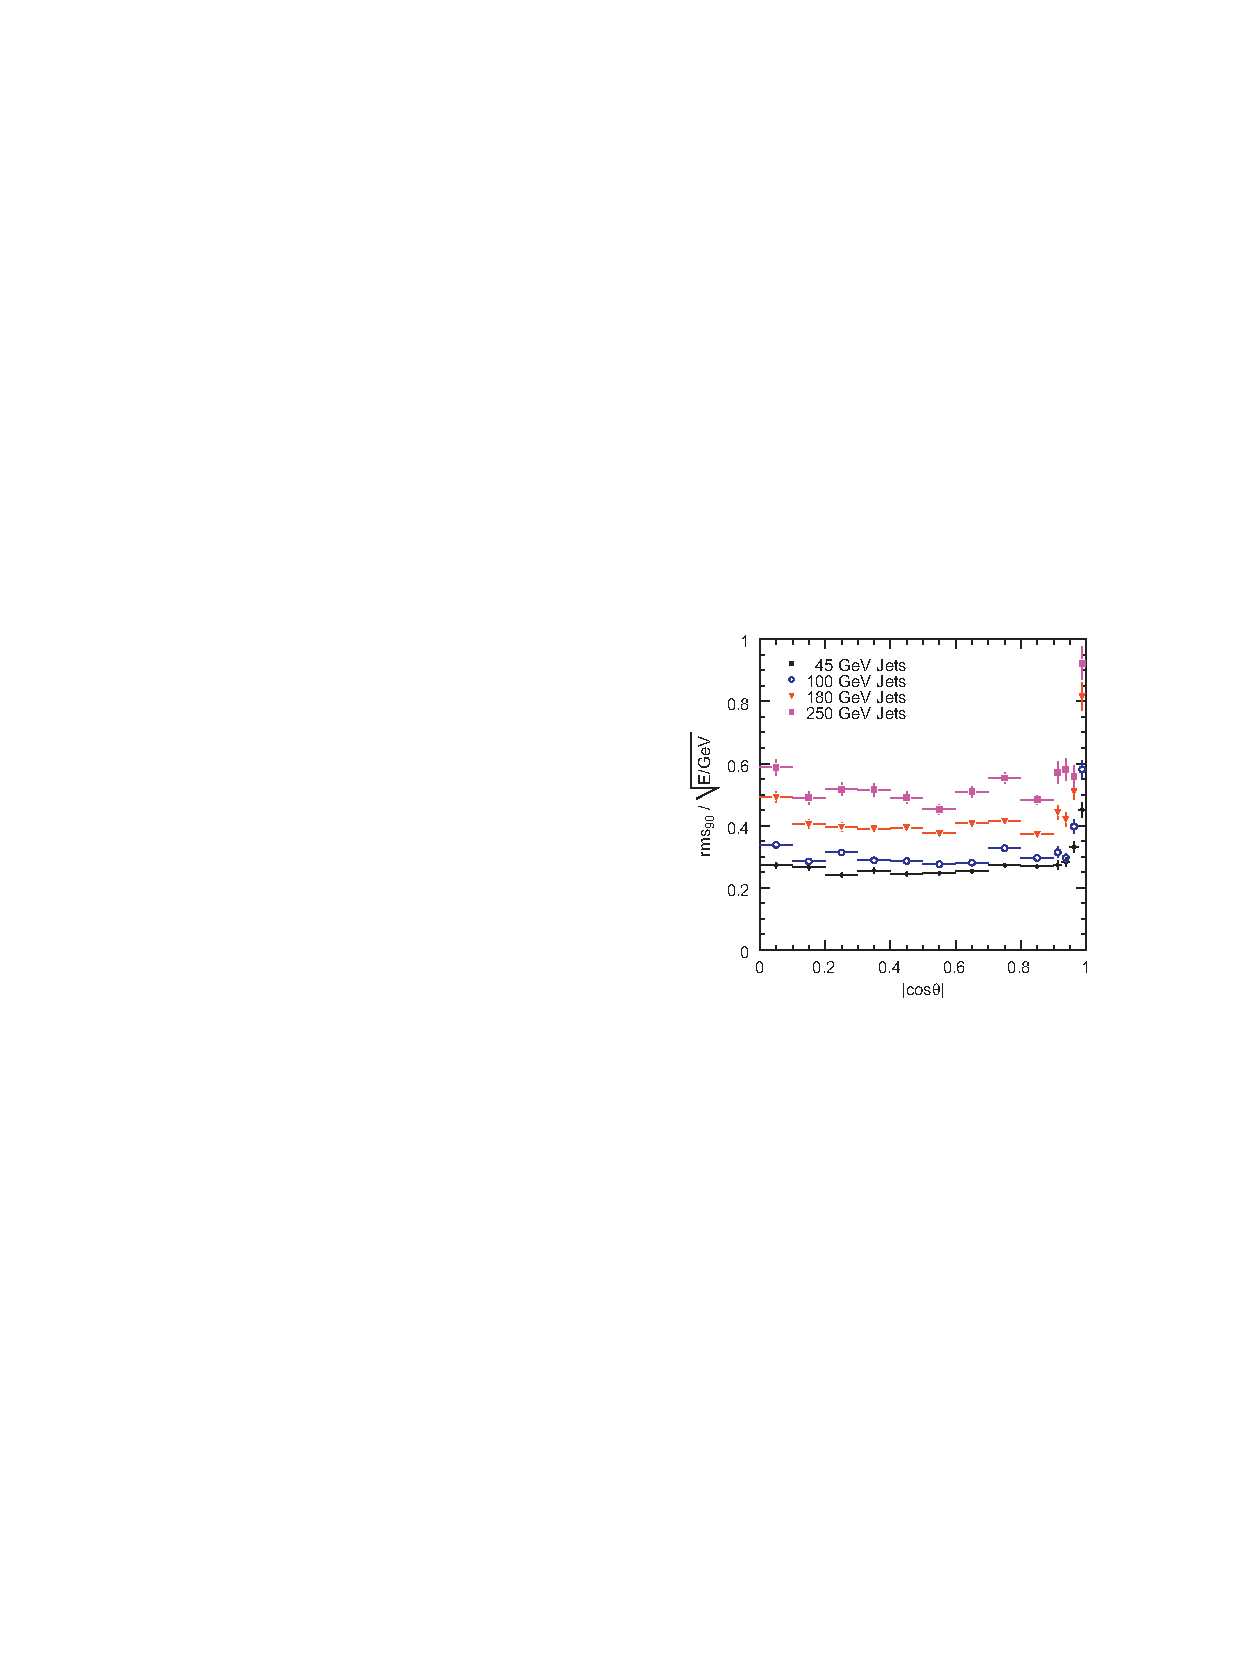
\includegraphics[width=0.55\textwidth]{ILD/JERangle}
\caption
{The jet energy resolution, defined as the \uprightMath{\alpha} in \uprightMath{\sigma / E = \alpha / \sqrt{E(GeV)}}, plotted versus angle of the \Zprime for four different values of \sqrtS, using \eeZuds, at barrel region of the detector. The figure is taken from \cite{Thomson:2009rp}.}
\label{fig:detectorJERangle}
\end{figure}

\end{comment}



\section{\CLICILD detector concept}


%he detector requirements for both the \ILC and \CLIC share similarities, as both detectors have similar physics goals. The detector requirements for the \CLIC are more stringent as the \CLIC detector needs to operate at a centre-of-mass energy of 3\,TeV. The most challenging prospect is the 0.5\,ns brunch structure and the background from \ggHad, which deposits 20\,TeV of energy in the calorimeter of the  entire 312 bunch trains. Therefore, an excellent time resolution for all detector components are needed, as well as a highly segmented calorimeter to keep each cell occupancies to an acceptable level. Here the requirement on the jet energy resolution at a future linear collider is presented in details.


There are two detector concepts studied in the \CLIC conceptual design report \cite{Linssen:2012hp}, the \CLICILD and the \CLICSiD concepts. The \CLICILD detector concept is based on the \ILD detector concept. \FIGURE{fig:CLIC_ILD} shows the longitudinal cross section of the \CLICILD detector. A comparison of key parameters for the \ILD and the \CLICILD detector concepts is shown in \Table{tab:ILDvsCLICILD}.

%As the \CLICILD is similar to the \ILD, only the differences are highlighted here.  

\begin{figure}[tbph]
\centering
    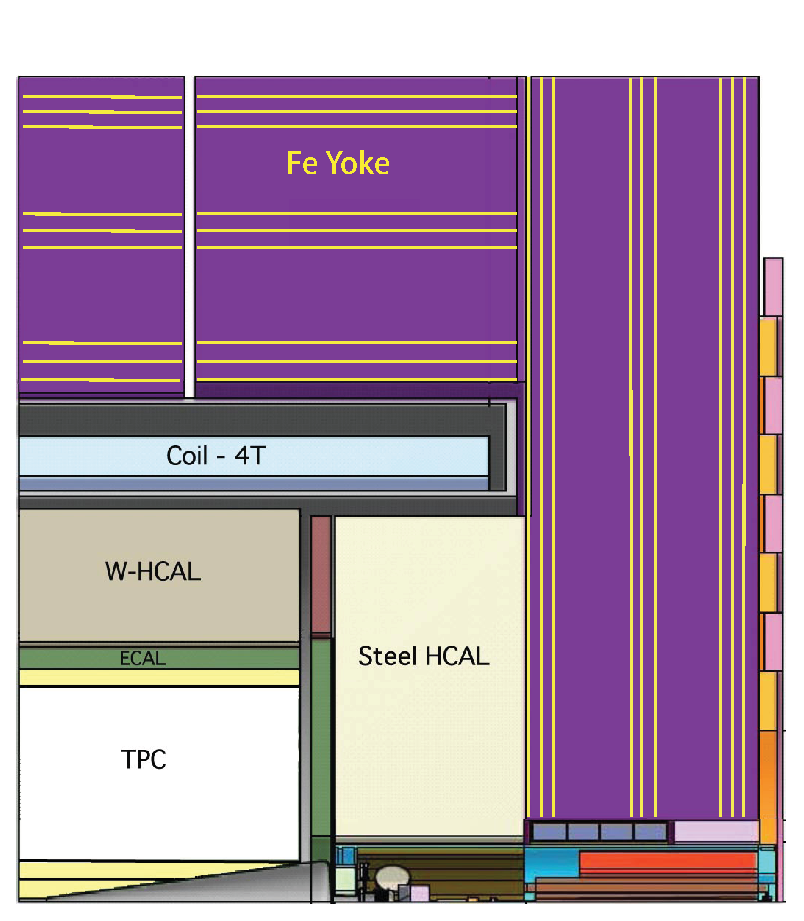
\includegraphics[width=0.8\textwidth]{ILD/CLIC_ILD}
\caption
{The longitudinal cross section of top quadrant the \CLICILD detector concept, taken from and \cite{Linssen:2012hp}. From interaction point (\IP) outwards, there is: a tracking system comprising a large time projection chamber (\TPC) augmented with silicon tungsten layers; highly granular electromagnetic calorimeters (\ECAL) and hadronic calorimeters (\HCAL);  forward calorimeters (\FCAL); a superconducting solenoid; and muon chambers embedded within the iron return yokes.}
    \label{fig:CLIC_ILD}
\end{figure}



For the \CLICILD vertex detector, the first layer is moved outwards by 15\,mm due to a larger high occupancy region with a higher centre-of-mass energy and a smaller beam jet. The detector is also required to provided time stamping at the  nanosecond level.

%, which needs different electronically components than those of the \ILD.

For the \CLICILD tracking detector, the same silicon$-$\TPC hybrid structure is used.  At \CLIC, it is challenging to use a \TPC to sperate two tracks in high-energy jets and to identify events in the collection of 312 bunch crossings in 156\,ns. The outer silicon tracking system is important to achieve a high momentum resolution at high centre-of-mass energy. The solid angle coverage of the tracking detector is $12\degree \lesssim \theta \lesssim 168\degree$

For the \CLICILD design, the same \ECAL as the \ILD is assumed, as the requirements of a \CLIC detector are satisfied by the  \ECAL design at the \ILD. 

%The increased centre-of-mass energy results in extra energy leakage. The leakage is controlled by the \HCAL.  Only a small fraction of particles are affected by the leakage.

For the \CLICILD \HCAL, extra layers are added to contain the hadronic shower for the  higher centre-of-mass energies of \CLIC. The increased thickness is justified by the simulation studies \cite{Linssen:2012hp}, where the jet energy resolution degrades quickly for a thinner \HCAL. To sustain the same inner bore radius as the \ILC detector solenoid, a more dense material, tungsten, is chosen as the absorber material in the \HCAL barrel.

The magnetic field is increased to 4\,T  for a better jet energy resolution \cite{Thomson:2009rp} at a higher centre-of-mass energy. Due to the different magnetic field strength, the iron yoke thickness is  increased to 230\,cm.

The \CLICILD adopts a similar very forward calorimetry system as that of the \ILD. The dimensions of the elements are changed due to a difference in the beam crossing angles (20\,mrad for \CLIC and 14\,mrad for the \ILC). A comparison of the key parameters for the \LumiCAL and the \BeamCAL at the \ILD and the \CLICILD is shown in \Table{tab:detectorForwardILDvsCLICILD}.

%Modifications to the design due to the \CLIC 3\,TeV centre-mass-of energy can be found in \cite{Linssen:2012hp}.






%Beam Calorimeter acceptance is defined as \absCosTheta is between  0.01 and 0.04\,rad and length in z direction is between 3181 and 3441\,mm. Luminosity Calorimeter acceptance is defined as \absCosTheta is between  0.038 and 0.11\,rad and length in z direction is between 2539 and 2714\,mm.



